\documentclass[compress]{beamer}




%%%%%%%%%%%%%%%%%%%%%%%%%%%
% LaTeX package inclusion %
%%%%%%%%%%%%%%%%%%%%%%%%%%%
\usepackage{times}
\usepackage{units}
\usepackage{mathrsfs}
\usepackage{diss} % defines \bv and some other stuff
\usepackage{subfigure}
\usepackage{multirow}
\usepackage{amsmath}
\usepackage{amssymb}
%\usepackage{algorithm}
%\usepackage{algorithmic}
\usepackage{hyperref}
\usepackage{listings}
\usepackage{movie15}
\usepackage{stmaryrd} % \llbracket
\graphicspath{{figs/}}



\usefonttheme[
  onlymath
]{serif} %onlymath option doesn't look too bad, eqns are more readable this way.

\definecolor{DarkGreen}{rgb}{0.13,0.55,0.13}
\definecolor{DarkRed}{rgb}{0.55,0.13,0.13}
\definecolor{mygray}{rgb}{0.5,0.5,0.5}
\definecolor{mymauve}{rgb}{0.58,0,0.82}
\setcounter{tocdepth}{1}


\usetheme{UB}
%\usetheme{nasatalk}

\definecolor{nasablue}{RGB}{0,96,169}
\definecolor{nasared}{RGB}{239,61,66}
\definecolor{orionblue}{RGB}{15,16,64}

%\usecolortheme{orchid} % white on dark block titles.  use w/ whale.
%\usecolortheme{whale} % darkest top titles, usually used by CFDLab presenters
\setbeamertemplate{itemize items}[circle]% Force any theme (eg Antibes) to use circle bullets
%\useinnertheme[shadow]{rounded} % Causes itemize blocks to have rounded corners & drop shadows
%\logo{\includegraphics[width=.5in]{common/rawfigs/word3}}
%\setbeamercolor{title}{fg=red!80!black,bg=red!20!white} %pink title!

\title[The \texttt{libMesh} Finite Element Library]{The \texttt{libMesh} Finite Element Library \\ \vspace{.5em} \emph{\large Object-Oriented High-Performance Computing}}
\author[P.~T.~Bauman]{Paul T. Bauman}
\institute[UB]{University at Buffalo, SUNY}
\date{March 25, 2015}

%\AtBeginSection[]{\frame{\tableofcontents[current]}}

% Dr. Carey's Notes:
% I had in mind some of the material we have in the Libmesh papers well
% as  from the perspective of:(1) a very knowlegable  developer,(2)
% installing an application with experience (3)  applying an
% application for parametric runs  with some examples. perhaps some of
% the issues encounter, as in all such codes like stopping criteria for
% adaptive refinement, selection of error indicators, flexibility in
% model adaption, ( adding terms, modifying constitutive models etc).
% perhaps something on the coarsening /refining ; one level exceptions
% etc. it would be helpful if you, Ben and Roy coordinated this.
% Someone should talk about PETSc, partitioning etc. Someone about
% memory restrictions etc. Strengths and limitations.  examples, couple
% of movies etc etc


% Abstract:
% This talk will focus on several of the practical aspects involved in
% using the LibMesh library for finite element analysis.  The topics
% covered will include: the steps in going from a mathematical model
% (PDE) to a working implementation (code), stopping criteria for
% adaptive refinement, the selection of error indicators, and model
% adaptation (adding terms, changing constitutive laws, etc).  The
% strengths, weaknesses, and current limitations of the library will
% be discussed in the same practical context.  Finally, some additional
% examples giving a flavor of the types of applications which have
% already been developed around the library will be given.
%\setbeamercovered{transparent}


\newcommand{\R}{\mathscr{R}}
\newcommand{\LibMesh}{\texttt{libMesh}}
\newcommand{\libmesh}{\texttt{libMesh}}
\newcommand{\emphcolor}[1]{\textcolor{nasablue}{#1}}
\newcommand{\royslide}[2]{\begin{frame} \frametitle{#1} #2 \end{frame}}
\newcommand{\royitemizebegin}[1]{\begin{block}{#1} \begin{itemize}}
\newcommand{\royitemizeend}{\end{itemize} \end{block}}

\begin{document}

\lstset{
  language=C++,
  basicstyle=\scriptsize\ttfamily,
  frame=none,
  commentstyle=\color{nasared},
  keywordstyle=\color{nasablue},   % keyword style
  numbers=none,                    % where to put the line-numbers; possible values are (none, left, right)
  numbersep=3pt,                   % how far the line-numbers are from the code
  numberstyle=\tiny\color{mygray}, % the style that is used for the line-numbers
  rulecolor=\color{black},         % if not set, the frame-color may be changed on line-breaks within not-black text
  showspaces=false,                % show spaces everywhere adding particular underscores; it overrides 'showstringspaces'
  showstringspaces=false,          % underline spaces within strings only
  showtabs=false,                  % show tabs within strings adding particular underscores
  stepnumber=2,                    % the step between two line-numbers. If it's 1, each line will be numbered
  stringstyle=\color{mymauve}      % string literal style
}


\begin{frame}
  \titlepage
\end{frame}



%===============================================================================
% Objectives
%===============================================================================
\begin{frame}
\frametitle{Course Objectives}

\begin{block}{Scope}
\begin{itemize}
\item Overview of libMesh:
        \begin{itemize}
        \item geometry data structures
        \item finite element data structures
        \item Building programs to solve finite element formulations
        \end{itemize}
\item Survey of more advanced features of library, if time
\end{itemize}
\end{block}

\begin{block}{Target Audience}
\begin{itemize}
\item PhD students/Postdocs with some knowledge of C++ and finite
  element methods
\end{itemize}
\end{block}

\begin{block}{Slides}
\begin{itemize}
\item Slides will be publicly available at: \url{https://github.com/libMesh/Documents}
\end{itemize}
\end{block}

\end{frame}

%===============================================================================
% Course Notes
%===============================================================================
\begin{frame}
\frametitle{Course Notes}

\begin{block}{This is for you!}
\begin{itemize}
\item Please stop me to ask questions
\item Please stop me to have a discussion
\item Please download the slides at your convenience
\end{itemize}
\end{block}

\begin{block}{Online Resources}
\begin{itemize}
\item \url{https://libmesh.github.io}
\item \href{mailto:libmesh-users@lists.sourceforge.net}{libmesh-users@lists.sourceforge.net}
\item \href{mailto:libmesh-devel@lists.sourceforge.net}{libmesh-devel@lists.sourceforge.net}
\item \textbf{PLEASE} don't email me directly about \texttt{libMesh}, use the list!
\end{itemize}
\end{block}

\end{frame}

\begin{frame}
  \frametitle{Originators of \texttt{libMesh}}
  \begin{block}{}
    \begin{itemize}
    \item 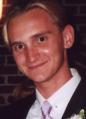
\includegraphics[scale=3]{benkirk} Benjamin S. Kirk, NASA Johnson Space Center
    \item 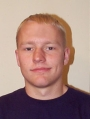
\includegraphics[scale=0.35]{jwpeterson} John W. Peterson, Idaho National Lab
    \item 
\includegraphics[scale=0.35]{roystgnr} Roy H. Stogner, University of Texas at Austin
    \end{itemize}
  \end{block}

\end{frame}

\frame
{
  \frametitle{Thanks to Dr.\ Graham F.\ Carey}

  \begin{columns}
    \begin{column}{.55\textwidth}
      \scriptsize
      \begin{quote}
        The original development team was heavily influenced by Professor Graham F. Carey, professor of aerospace engineering and engineering mechanics at The University of Texas at Austin, director of the ICES Computational Fluid Dynamics Laboratory, and holder of the Richard B. Curran Chair in Engineering.

        Many of the technologies employed in libMesh were implemented because Dr. Carey taught them to us, we went back to the lab, and immediately began coding. In a very real way, he was ultimately responsible for this library that we hope you may find useful, despite his continued insistence that ``no one ever got a PhD from here for writing a code.''
      \end{quote}
\normalsize
    \end{column}
    \begin{column}{.45\textwidth}
      \includegraphics[width=\textwidth]{grahamcarey}
    \end{column}
  \end{columns}
}

% The optional argument [<+->] means everything on the frame will be displayed incrementally.


\begin{frame}[shrink]
  \begin{block}{Code Contributors}
    \scriptsize
    \begin{center}
      \begin{tabular}{|l|l|} \hline
        Benjamin S. Kirk & benkirk \\
        Bill Barth       & bbarth \\
        Cody Permann     & permcody \\
        Daniel Dreyer    & ddreyer \\
        David Andrs      & andrsd \\
        David Knezevic   & knezed01 \\
        Derek Gaston     & friedmud \\
        Dmitry Karpeev   & karpeev \\
        Florian Prill    & fprill \\
        Jason Hales      & jasondhales \\
        John W. Peterson & jwpeterson \\
        Paul T. Bauman   & pbauman \\
        Roy H. Stogner   & roystgnr \\
        Steffen Petersen & spetersen \\
        Sylvain Vallaghe & svallagh \\
        Tim Kroeger      & sheep\_tk \\
        Truman Ellis     & trumanellis \\
        Wout Ruijter     & woutruijter \\ \hline
      \end{tabular}
    \end{center}
    \begin{itemize}
      \item Thanks to Wolfgang Bangerth and the \texttt{deal.II} team for initial technical inspiration.
      \item Also, thanks to Jed Brown, Robert McLay, \& many others for discussions over the years.
    \end{itemize}
  \end{block}
\end{frame}



%=================================================================
% Outline
%=================================================================
%\section{Introduction}
%% Auto-generate the TOC slide(s)
\begin{frame}
  \tableofcontents[currentsection]
  %\tableofcontents
\end{frame}

\section*{Outline}% Make it easy to jump to this page in the PDF

% Auto-generate the TOC slide(s)
\begin{frame}
  \frametitle{Outline}
  %\tableofcontents[currentsection]
  \tableofcontents
\end{frame}




\section{Introduction}
%%%%%%%%%%%%%%%%%%%%%%%%%%%%%%%%%%%%%%%%%%%%%%%%%
\commentout{
\frame
{
  \frametitle{Background}

  \begin{itemize}
  \item Modern simulation software is \emphcolor{complex}:
    \begin{itemize}
    \item Implicit numerical methods
    \item Massively parallel computers
    \item Adaptive methods
    \item Multiple, coupled physical processes
    \end{itemize}
    %\pause
  \item There are a host of existing software libraries that excel at treating various aspects of this complexity.
  \item Leveraging existing software whenever possible is the most efficient way to manage this complexity.

  \end{itemize}
}




%%%%%%%%%%%%%%%%%%%%%%%%%%%%%%%%%%%%%%%%%%%%%%%%%
\frame
{
  \frametitle{Background}

  \begin{itemize}
  \item Modern simulation software is \emphcolor{multidisciplinary}:
    \begin{itemize}
    \item Physical Sciences
    \item Engineering
    \item Computer Science
    \item Applied Mathematics
    \item \ldots
    \end{itemize}
  \item It is not reasonable to expect a single person to have all the necessary skills for developing \& implementing high-performance numerical algorithms on modern computing architectures.
  \item Teaming is a prerequisite for success.
  \end{itemize}
}
} % commentout


 

%%%%%%%%%%%%%%%%%%%%%%%%%%%%%%%%%%%%%%%%%%%%%%%%%
\frame
{
  \frametitle{Background}                 
  \begin{itemize}
    \item A large class of problems are amenable to \emphcolor{mesh based} simulation techniques.
      %% \begin{columns}[t]
      %%   \column{.5\textwidth}        
      %%   \fbox{\includegraphics[viewport=140 420 400 685,clip=true,height=1in]{domain2/domain2_input}}
      %%   \column{.5\textwidth}
      %%   \fbox{\includegraphics[height=1in,angle=-90]{discretized_domain}}
      %% \end{columns}
    \item Consider some of the major components such a simulation:
      \pause
      \begin{enumerate}
        \item Read the mesh from file
        \item Initialize data structures
        \item Construct a discrete representation of the governing equations
        \item Solve the discrete system
        \item Write out results
        \item Optionally estimate error, refine the mesh, and repeat
      \end{enumerate}

    \pause
    \item With the exception of step 3, the rest is \emph{independent} of the class of problems being solved.
    \pause
    \item This allows the major components of such a simulation to be abstracted \& implemented in a reusable software library.
  \end{itemize}
}


 

\subsection{The \libmesh{} Software Library}
%%%%%%%%%%%%%%%%%%%%%%%%%%%%%%%%%%%%%%%%%%%%%%%%%
\frame
{
  \frametitle{The \libmesh{} Software Library}
  \begin{itemize}
    \item In 2002, the \libmesh{} library began with these ideas in mind.
    \item Primary goal is to provide data structures and algorithms that can be shared by disparate physical applications, that may need some combination of
      \begin{itemize}
      \item Implicit numerical methods
      \item Adaptive mesh refinement techniques
      \item Parallel computing
      \end{itemize}
    \item Unifying theme: \emphcolor{mesh-based simulation of partial differential equations (PDEs)}.
  \end{itemize}
}



 

\subsection{Software Reusability}
%%%%%%%%%%%%%%%%%%%%%%%%%%%%%%%%%%%%%%%%%%%%%%%%%
\frame
{
  \frametitle{The \libmesh{} Software Library}

\begin{columns}
\column{.5\textwidth}
  \begin{block}{\libMesh{} Goals}
    \begin{itemize}
      \item Use by students, researchers, scientists, and engineers as a tool for \emphcolor{developing simulation codes} or as a tool for \emphcolor{rapidly implementing a numerical method}.
      \item \libMesh{} is not an application code.
      \item It does not ``solve problem XYZ.''
        \begin{itemize}
          \item It helps users develop applications to solve XYZ,
              quickly, with advanced algorithms on HPC platforms.
        \end{itemize}
      %\item It was initially targeted for finite element based simulations, but has been used for finite volume discretizations as well.
    \end{itemize}    
  \end{block}
\column{.45\textwidth}
  \begin{center}
    \includegraphics[width=.9\textwidth]{mytreeandroots_allnames}
  \end{center}
\end{columns}
} 


\begin{frame}{libMesh Community}
\begin{columns}
\column{.4\textwidth}
\begin{block}{Scope}
\begin{itemize}
\item Free, Open source
\begin{itemize}
\item LGPL2 for core
\end{itemize}
\item 70 Ph.D.\ theses, 721 papers (134 in 2017)
\item $\sim10$ current developers
\item $110-240$ current users?
\end{itemize}
\end{block}

\column{.6\textwidth}
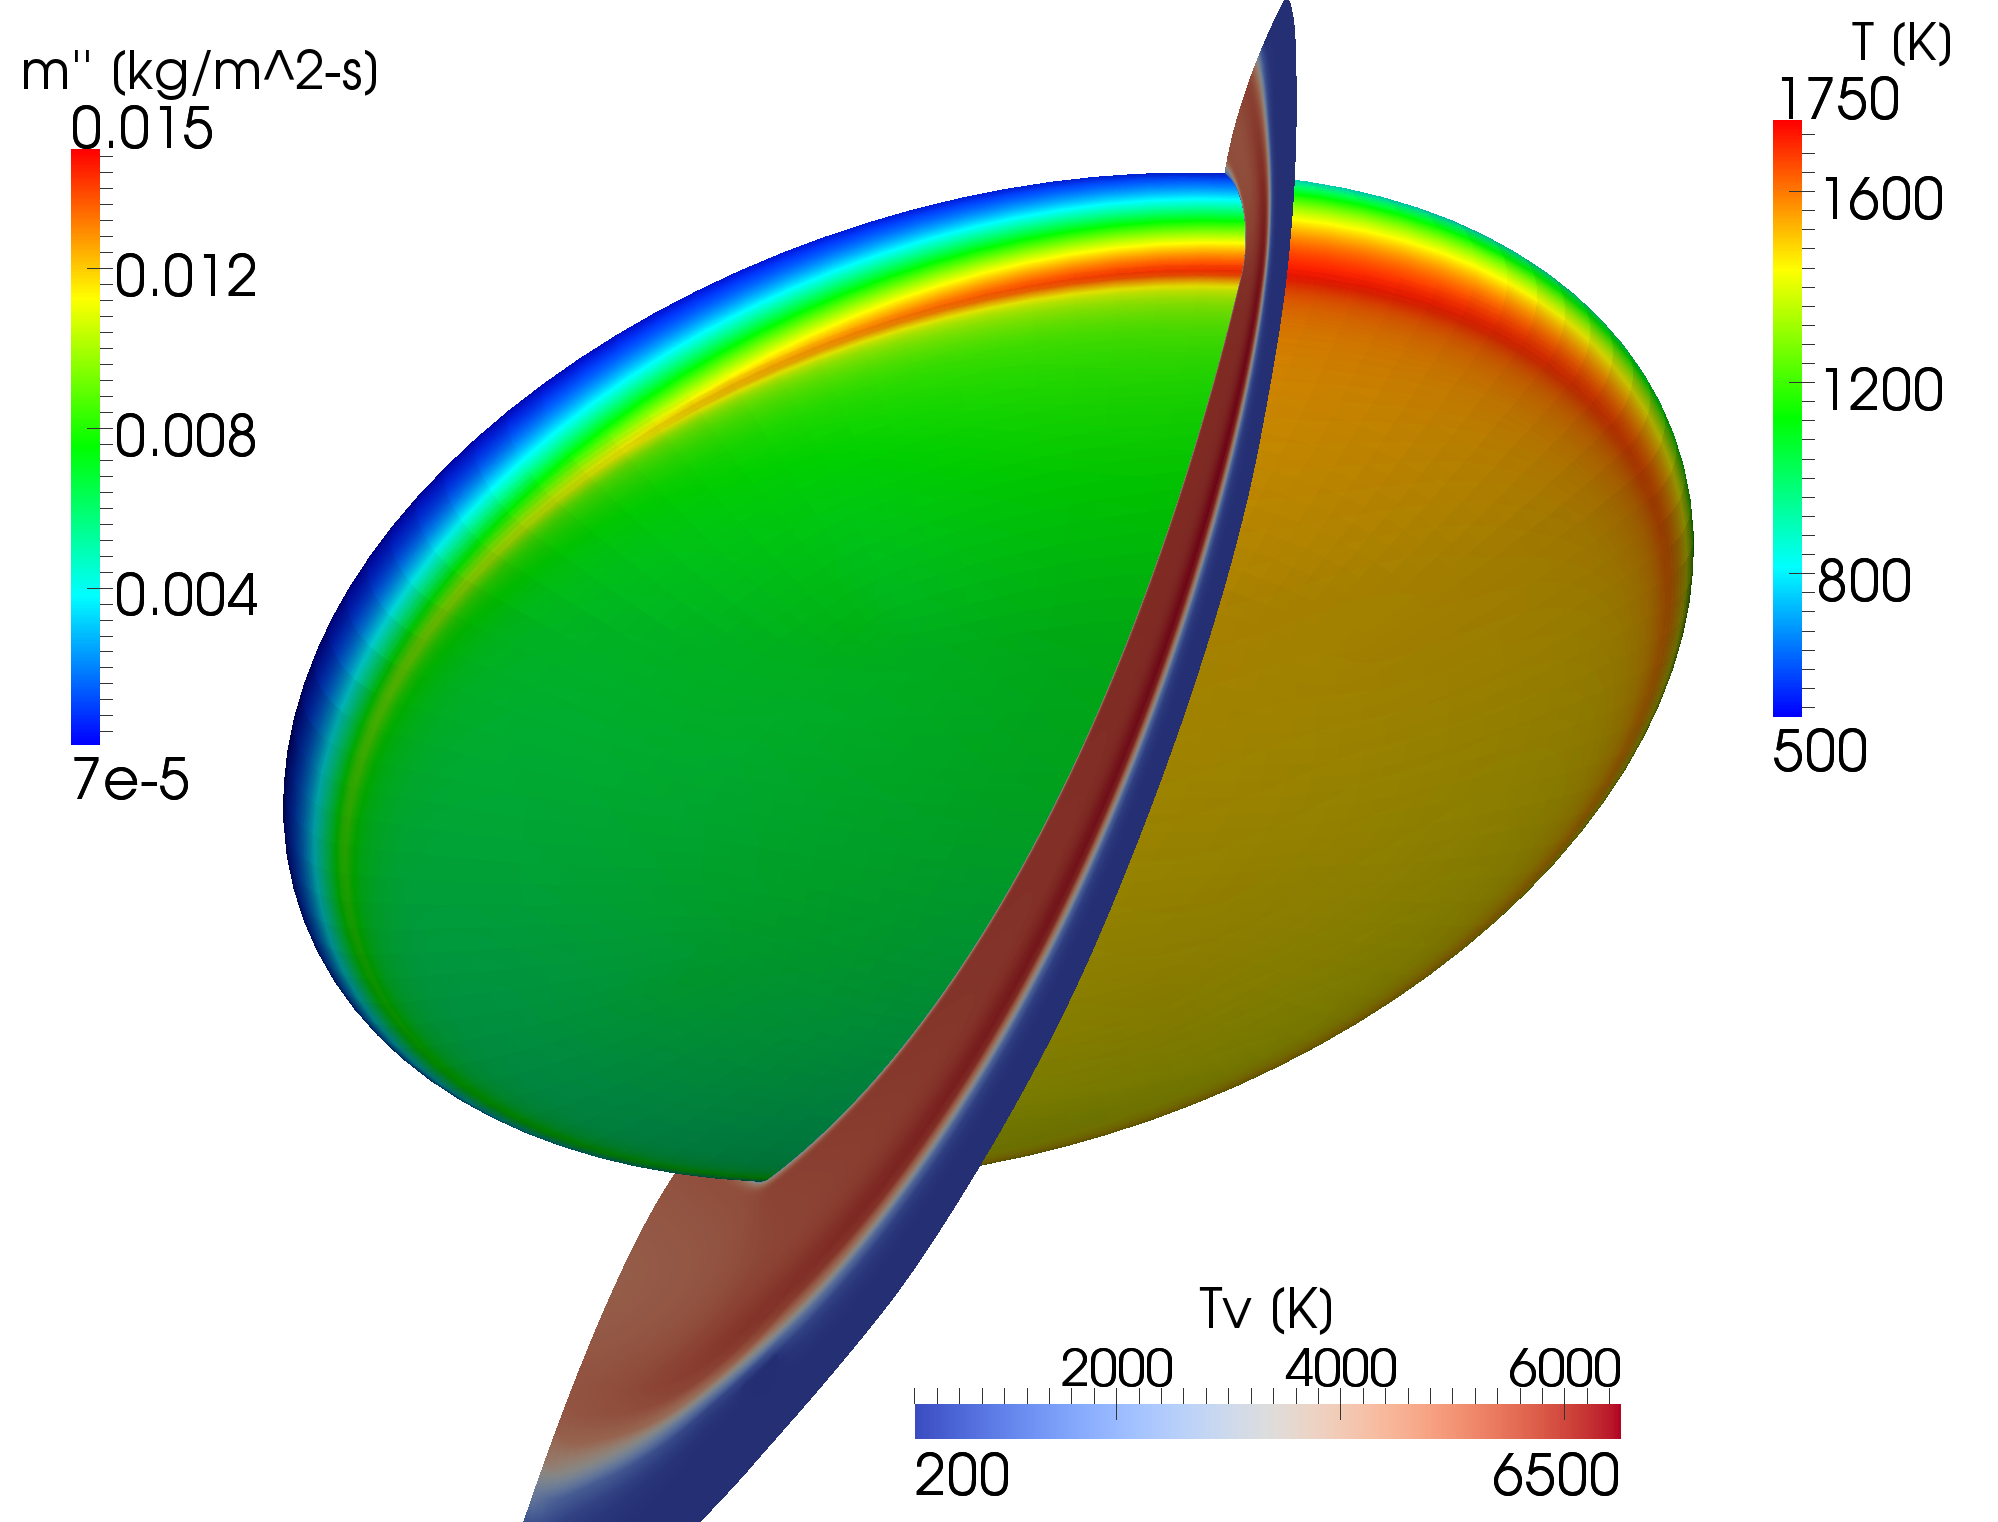
\includegraphics[width=.45\textwidth]{ablating_hs_wbg}
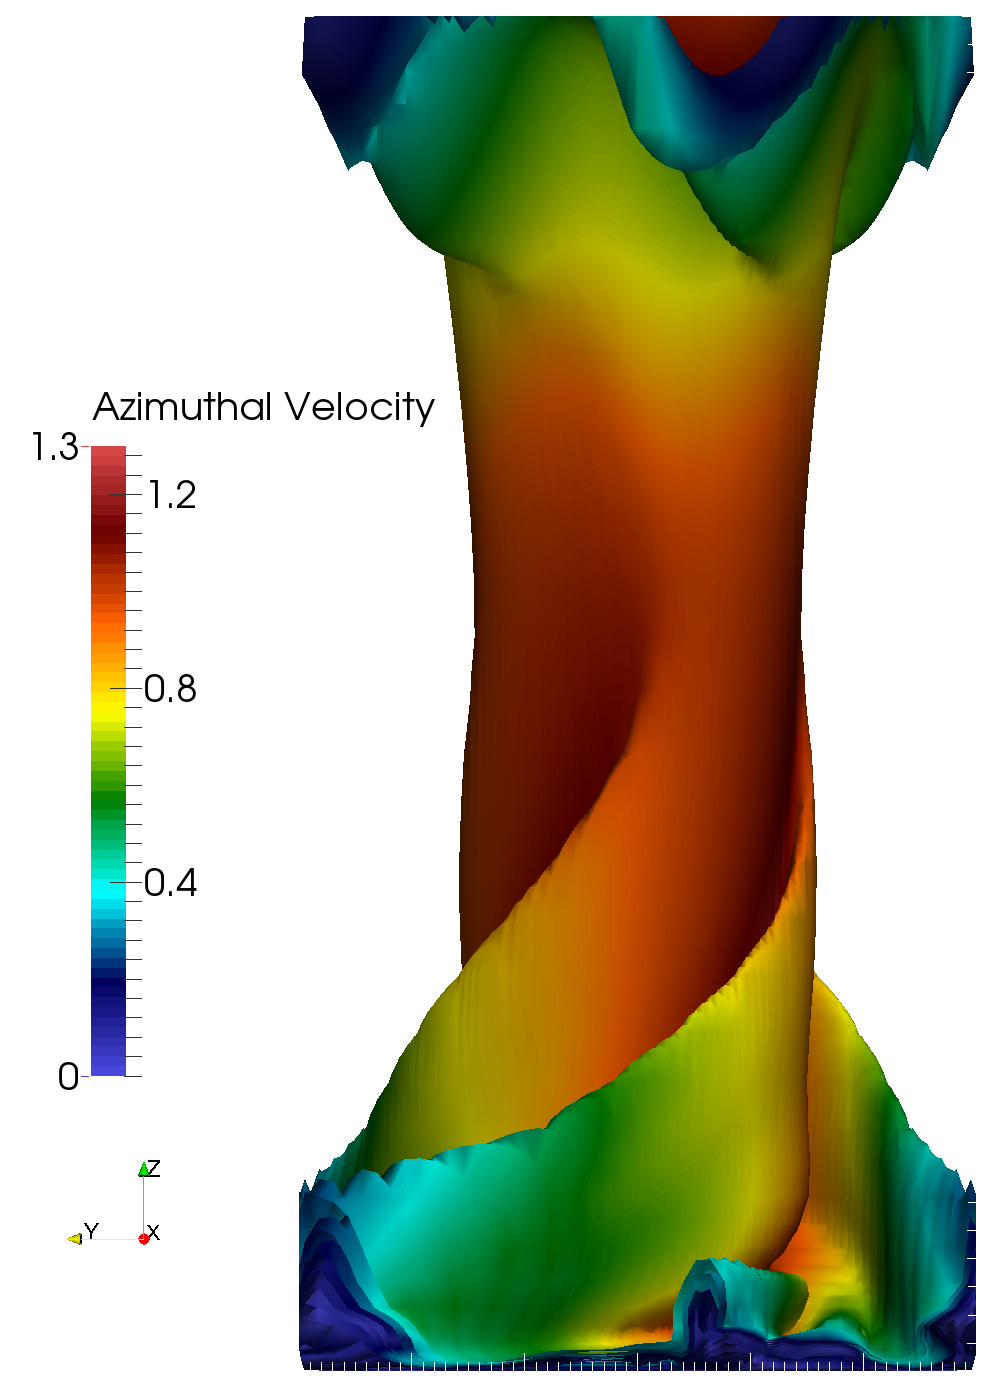
\includegraphics[width=.25\textwidth]{sov}
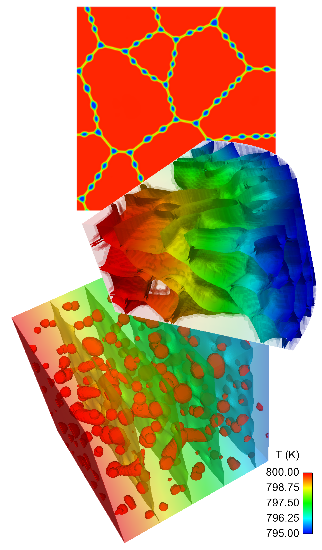
\includegraphics[width=.3\textwidth]{marmot1b}
\end{columns}

\begin{columns}
\column{.35\textwidth}
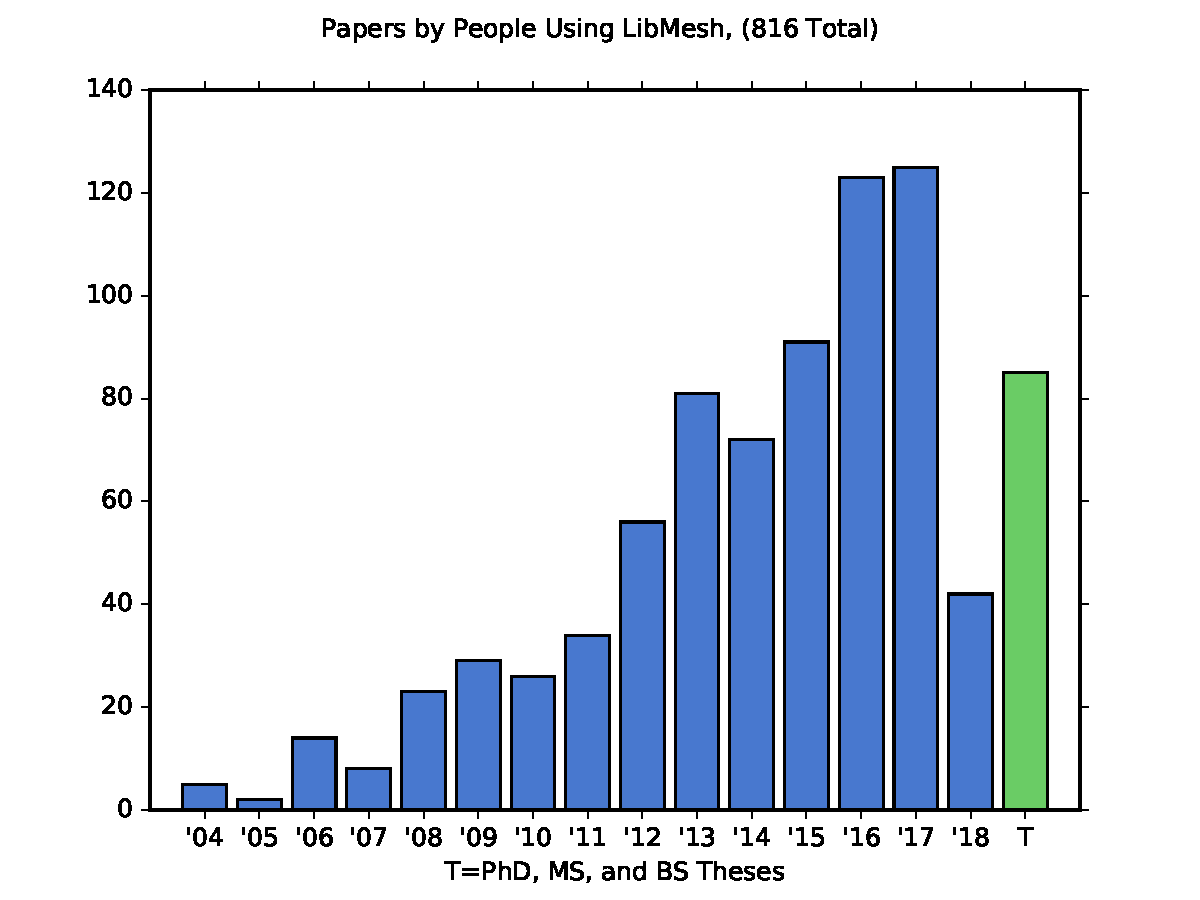
\includegraphics[width=\textwidth]{libmesh_citations}

\column{.65\textwidth}
\begin{block}{Challenges}
\begin{itemize}
\item Radically different application types
\item Widely dispersed core developers
\begin{itemize}
\item INL, UT-Austin, U.Buffalo, JSC, MIT, Harvard, Argonne
\end{itemize}
\item OSS, commercial, private applications
\end{itemize}
\end{block}
\end{columns}

\end{frame}





%\subsection*{Non-Trivial Applications}
\begin{frame}%[t]
%  \frametitle{Weighted Residual Connection}
  %\begin{block}{}
  \begin{itemize}%[<+->]
  \item{\libMesh{} provides several of the tools necessary to construct
    these systems, but it is not specifically written to solve any one
    problem.}

  \item{First, a few of the non-trivial applications which have been built on
    top of the library.}
    
%%   \item{In each case, the matrix $A$ is the ``Jacobian''
%%     operator, and the right-hand side vector $b$ is the
%%     weighted residual itself.}

    %% 	\item{This is true even in the case of linear $\R( u )$, since
    %% 	  in this case the linearized operator is
    %% 	  \begin{eqnarray}
    %% 	    \nonumber
    %% 	    \R'( u )w &:=& \lim_{\varepsilon\rightarrow 0}
    %% 	    \frac{\R(u+\varepsilon w) - \R(u)}{\varepsilon} \\
    %% 	    \nonumber
    %% 	    &=& \R(w)
    %% 	  \end{eqnarray}
    %% 	}
  \end{itemize}
%\end{block}
\end{frame}	  

%\subsection*{Natural Convection}
\begin{frame}[t]
  \begin{center}
    \includegraphics[width=.45\textwidth]{part_trans}
    %\\
    \includegraphics[width=.45\textwidth]{streamtraces}
  \end{center}
  \begin{block}{}
    \begin{itemize}
    \item{
      Tetrahedral mesh of ``pipe'' geometry.
      Stream ribbons colored by temperature.
      }
      \end{itemize}
  \end{block}
\end{frame}

%\subsection*{Surface-Tension-Driven Flow}
\begin{frame}[t]
  \begin{center}
    \includegraphics[width=.6\textwidth]{rbm_adapt_soln}    
  \end{center}

  \begin{block}{}
    \begin{itemize}
    \item{Adaptive grid solution shown
      with temperature contours and velocity vectors.
      }
      \end{itemize}
  \end{block}
\end{frame}

%\subsection*{Double-Diffusive Convection}
\begin{frame}[t]
  \begin{center}
    \includegraphics[width=.6\textwidth]{dd}    
  \end{center}

  \begin{block}{}
    \begin{itemize}
    \item{Solute contours: a plume of
      warm, low-salinity fluid is convected upward through a porous medium.
      }
      \end{itemize}
  \end{block}
\end{frame}



%\subsection*{Tumor Angiogenesis}
\begin{frame}[t]
  \begin{center}
    \includegraphics[width=.6\textwidth]{tumor_model}    
  \end{center}

  \begin{block}{}
    \begin{itemize}
    \item{%Tumor angiogenesis model simulation.
      The tumor secretes
      a chemical which stimulates blood vessel formation.
      }
      \end{itemize}
  \end{block}
\end{frame}



%\subsection*{Phase Separation}
\begin{frame}[t]
  \begin{center}
    \includegraphics[width=.3\textwidth]{ch3D02-006}    
    \includegraphics[width=.3\textwidth]{ch3D02-024}    
    \includegraphics[width=.3\textwidth]{ch3D02-096}    
  \end{center}

  \begin{block}{}
    \begin{itemize}
    \item{%Tumor angiogenesis model simulation.
      Directed pattern self-assembly in spinodal decomposition of binary
mixture
      }
      \end{itemize}
  \end{block}
\end{frame}



%\subsection*{Compressible Flow}

\frame
{
  \frametitle{Compressible Shocked Flow}
  \begin{itemize}[<+->]
    \item Original compressible flow code written by Ben Kirk utilizing \libMesh{}.
      \begin{itemize}[<+->]
      \item Solves both Compressible Navier Stokes and Inviscid Euler.
      \item Includes both SUPG and a shock capturing scheme.
      \end{itemize}
    \item Original redistribution code written by Larisa Branets.
      \begin{itemize}[<+->]
      \item Simultaneous optimization of element shape and size.
      \item Directable via user supplied error estimate.
      \end{itemize}
    \item Integration work done by Derek Gaston.
      \begin{itemize}[<+->]
      \item Combination of redistribution, $h$ refinement.
      \item Applicable to other problem classes.
      \end{itemize}
  \end{itemize}
}

\frame
{
  \frametitle{Problem Specification}
  \begin{itemize}[<+->]
    \item The problem studied is that of an oblique shock generated by a $10^o$ wedge angle. 
      \begin{itemize}[<+->]
      \item This problem has an exact solution for density which is a step function.
      \item Utilizing \libMesh{}'s exact solution capability the exact
$L_2$ error can be solved for.
      \item The exact solution is shown below:
        \begin{figure}
          \begin{center}
            \includegraphics[viewport=20 10 660 600,clip=true,width=.4\textwidth]{shock.pdf}
          \end{center}
        \end{figure}
    \end{itemize}
  \end{itemize}
}

\frame
{
  \frametitle{Uniformly Refined Solutions}
  \begin{itemize}[<+->]
  \item For comparison purposes, here is a mesh and a solution after 1 uniform refinement with 10890 DOFs.
    \begin{figure}[!htb]
      \begin{center}
        \subfigure[Mesh after 1 uniform refinement.]{\label{fig:fob_uniform_2_mesh}\includegraphics[viewport=110 30 600 550,clip=true,width=.42\textwidth]{fob_uniform_2_mesh.pdf}}
        \subfigure[Solution after 1 uniform refinement.]{\label{fig:fob_uniform_2_sol}\includegraphics[viewport=110 30 600 520,clip=true,width=.42\textwidth]{fob_uniform_2_sol.pdf}}
      \end{center}
    \end{figure}
  \end{itemize}
}

\frame
{
  \frametitle{H-Adapted Solutions}
  \begin{itemize}[<+->]
    \item A flux jump indicator was employed as the error indcator along with a statistical flagging scheme.
    \item Here is a mesh and solution after 2 adaptive refinements containing 10800 DOFs:
      \begin{figure}[!htb]
        \begin{center}
          \subfigure[Mesh, 2 refinements]{\label{fig:fob_adapt_3_mesh}\includegraphics[viewport=110 30 600 550,clip=true,width=.42\textwidth]{fob_adapt_3_mesh.pdf}}
          \subfigure[Solution]{\label{fig:fob_adapt_3_sol}\includegraphics[viewport=110 30 600 520,clip=true,width=.42\textwidth]{fob_adapt_3_sol.pdf}}
        \end{center}
      \end{figure}
  \end{itemize}
}

\frame
{
  \frametitle{Redistributed Solutions}
  \begin{itemize}[<+->]
    \item Redistribution utilizing the same flux jump indicator.
      \begin{figure}[!htb]
        \begin{center}
          \subfigure[Mesh, 8 redistribution steps]{\label{fig:fob_redist_adapt_8_mesh}\includegraphics[viewport=110 30 600 550,clip=true,width=.42\textwidth]{fob_redist_adapt_8_mesh.pdf}}
          \subfigure[Solution]{\label{fig:fob_redist_adapt_8_sol}\includegraphics[viewport=110 30 600 520,clip=true,width=.42\textwidth]{fob_redist_adapt_8_sol.pdf}}
        \end{center}
      \end{figure}
  \end{itemize}
}

\frame
{
  \frametitle{Redistributed and Adapted}
  \begin{itemize}[<+->]
    \item Now combining the two, here are the mesh and solution after 2 adaptations beyond the previous redistribution containing 10190 DOFs.
      \begin{figure}[!htb]
        \begin{center}
          \subfigure[Mesh, 2 refinements]{\label{fig:fob_redist_adapt_10_mesh}\includegraphics[viewport=110 30 600 550,clip=true,width=.42\textwidth]{fob_redist_adapt_10_mesh.pdf}}
          \subfigure[Solution]{\label{fig:fob_redist_adapt_10_sol}\includegraphics[viewport=110 30 600 520,clip=true,width=.42\textwidth]{fob_redist_adapt_10_sol.pdf}}
        \end{center}
      \end{figure}
  \end{itemize}
}

\frame
{
  \frametitle{Solution Comparison}
  \begin{itemize}[<+->]
    \item For a better comparison here are 3 of the solutions, each with around 11000 DOFs:
      \begin{figure}[!htb]
        \begin{center}
          \subfigure[Uniform.]{\label{fig:fob_uniform_2_sol}\includegraphics[viewport=110 30 600 520,clip=true,width=.3\textwidth]{fob_uniform_2_sol.pdf}}
          \subfigure[Adaptive.]{\label{fig:fob_adapt_3_sol}\includegraphics[viewport=110 30 600 520,clip=true,width=.3\textwidth]{fob_adapt_3_sol.pdf}}
          \subfigure[R + H.]{\label{fig:fob_redist_adapt_10_sol}\includegraphics[viewport=110 30 600 520,clip=true,width=.3\textwidth]{fob_redist_adapt_10_sol.pdf}}
        \end{center}
      \end{figure}
  \end{itemize}
}

\frame
{
  \frametitle{Error Plot}
  \begin{itemize}[<+->]
    \item \libMesh{} provides capability for computing error norms against an exact solution.
    \item The exact solution is not in $H^1$ therefore we only obtain
the $L_2$ convergence plot:
      \begin{figure}[!htb]
      \begin{center}
        \subfigure[LogLog plot of L2 vs DOFs.]{\label{fig:fob_l2}\includegraphics[viewport=0 10 600 400,clip=true,width=.7\textwidth]{fob_l2.pdf}}
      \end{center}
      \end{figure}
  \end{itemize}
}

\frame
{
  %\frametitle{Other Compressible Flow Examples}
    \begin{figure}[!htb]
      \begin{center}
        \subfigure{\label{fig:fob_uniform_2_sol}\includegraphics[width=.4\textwidth]{Hypersonic_cow_mach}}
        \subfigure{\label{fig:fob_adapt_3_sol}\includegraphics[width=.4\textwidth]{Benkirk_orbiter_reentry_side_view}}
        \subfigure{\label{fig:fob_redist_adapt_10_sol}\includegraphics[width=.4\textwidth]{Benkirk_schlieren}}
        \subfigure{\label{fig:fob_redist_adapt_10_sol}\includegraphics[width=.4\textwidth]{Benkirk_double_cone_M}}
      \end{center}
    \end{figure}
}

\section{Motivation}
\subsection{Application Results}



%%%%%%%%%%%%%%%%%%%%%%%%%%%%%%%%%%%%%%%%%%%%%%%%%
\frame
{
  \Large
  \begin{block}{}
    \center{Results from Physics Applications built}
    \center{on top of \bf{\libmesh{}}}
  \end{block}
}



%%%%%%%%%%%%%%%%%%%%%%%%%%%%%%%%%%%%%%%%%%%%%%%%%
\frame
{
  \frametitle{FIN-S: Fully Implicit Navier-Stokes}

  \begin{columns}
    \begin{column}{0.45\textwidth}
      \begin{itemize}
      \item Kirk, Stogner, Bauman, Oliver, Computers \& Fluids, 2014
      \item Application for high-speed (including reentry)
        compressible flows in thermochemical nonequilibrium
      \item Including AMR capabilities
      \item Fully implicit coupling with surface response models
      \end{itemize}
    \end{column}
    %
    \begin{column}{0.45\textwidth}
      \begin{center}
        \only<1>{\includegraphics[height=\linewidth]{nosetip/smeared.png}}
        \only<2>{\includegraphics[height=\linewidth]{nosetip/amr.png}}
        \only<3>{\includegraphics[height=\linewidth]{nosetip/smeared.pdf}}
        \only<4>{\includegraphics[height=\linewidth]{nosetip/amr.pdf}}
        \only<5>{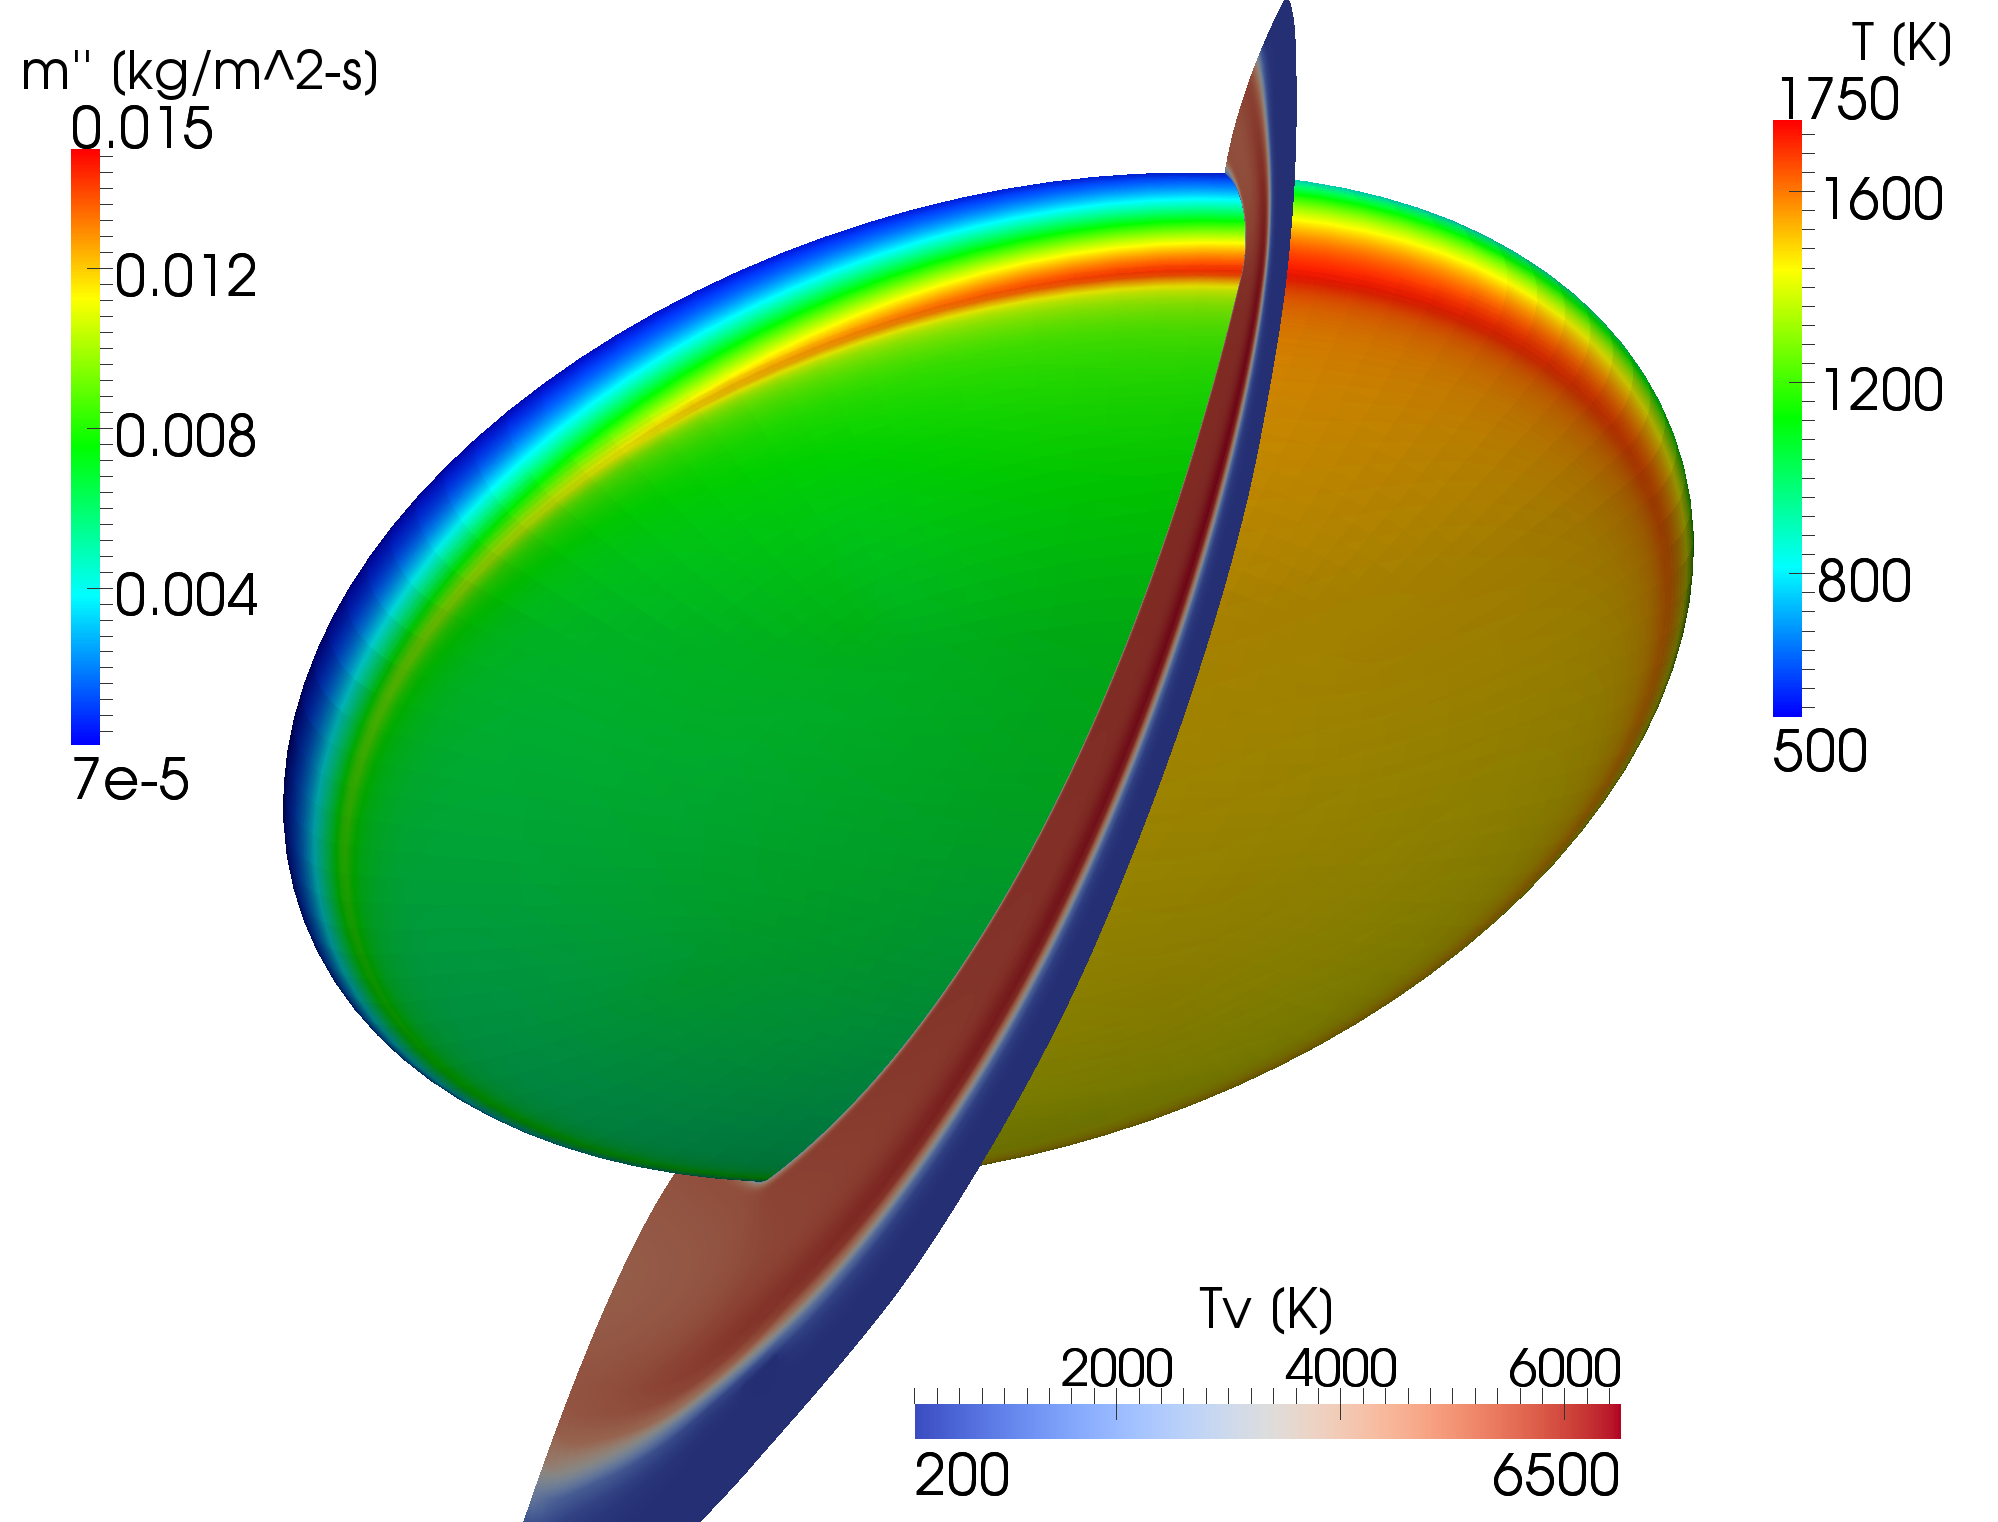
\includegraphics[height=\linewidth]{ablating_hs_wbg}}
      \end{center}
    \end{column}
  \end{columns}
}
%===============================================================================
% NEW SLIDE
%===============================================================================
\frame
{
  \frametitle{FIN-S: Arcjet Nozzle Calculation}
  \begin{center}
      
    \only<1>{\includegraphics[width=0.95\linewidth,trim=4px 4px 4px 4px,clip]{arcjet/viz/T}}
    
    \only<2>{\includegraphics[width=0.95\linewidth,trim=4px 4px 4px 4px,clip]{arcjet/viz/M}}
    
  \end{center}
}



%===============================================================================
% NEW SLIDE
%===============================================================================
%% \frame
%% {
%%   \frametitle{Arcjet Nozzle Calculation}
%%   \begin{center}

%%     \only<1>{\includegraphics[width=.95\textwidth,trim=4px 4px 4px 4px,clip]{arcjet/data/nozzle/P-streamlines.png}}

%%     \only<2>{\includemovie[autoplay,loop,text={\includegraphics[width=.95\textwidth,trim=4px 4px 4px 4px,clip]{arcjet/data/nozzle/P-streamlines.png}}]{.95\textwidth}{}{rawfigs/arcjet/data/nozzle/P.avi}}

%%   \end{center}
%% }



%===============================================================================
% NEW SLIDE
%===============================================================================
%% \frame
%% {
%%   \frametitle{Coupled Pyrolysis, Temperature}
%%   \begin{center}

%%     \only<1>{\includegraphics[height=.85\textheight]{arcjet/data/coupled/T.png}}

%%     \only<2>{\includemovie[autoplay,loop,text={\includegraphics[height=.85\textheight]{arcjet/data/coupled/T.png}}]{}{.85\textheight}{rawfigs/arcjet/data/coupled/T.avi}}

%%   \end{center}
%% }


%===============================================================================
% NEW SLIDE
%===============================================================================
%% \frame
%% {
%%   \frametitle{Coupled Pyrolysis, Pyrolysis gas mass flux, $\dot{m}$}
%%   \begin{center}

%%     \only<1>{\includegraphics[height=.85\textheight]{arcjet/data/coupled/mdotzoom.png}}

%%     \only<2>{\includemovie[autoplay,loop,text={\includegraphics[height=.85\textheight]{arcjet/data/coupled/mdotzoom.png}}]{}{.85\textheight}{rawfigs/arcjet/data/coupled/mdotzoom.avi}}

%%   \end{center}
%% }



%% \frame
%% {
%%   \frametitle{The MOOSE Framework - Gaston et al., INL}
%%   \begin{center}
%%     \fbox{\includegraphics[page=1,height=0.8\textheight]{Gaston/talk}}
%%   \end{center}
%% }



\frame
{
  \frametitle{The MOOSE Framework - Gaston et al., INL}
  \begin{center}
    \fbox{\includegraphics[page=2,height=0.8\textheight]{Gaston/talk}}
  \end{center}
}



%% \frame
%% {
%%   \frametitle{The MOOSE Framework - Gaston et al., INL}
%%   \begin{center}
%%     \fbox{\includegraphics[page=4,height=0.8\textheight]{Gaston/talk}}
%%   \end{center}
%% }



\frame
{
  \frametitle{The MOOSE Framework - Gaston et al., INL}
  \begin{center}
    \fbox{\includegraphics[page=22,height=0.8\textheight]{Gaston/talk}}
  \end{center}
}

\frame
{
  \frametitle{Coupled Thermal/Solid Mechanics}
  \begin{center}

    \only<1>{\includegraphics[height=.85\textheight]{Gaston/pgc.png}}

    \only<2>{\includemovie[autoplay,loop,text={\includegraphics[height=.85\textheight]{Gaston/pgc.png}}]{}{.85\textheight}{Gaston/pgc.avi}}

  \end{center}
}


%===============================================================================
% New Slide
%===============================================================================
\begin{frame}
\frametitle{\texttt{GRINS}}

\begin{block}{\url{https://github.com/grinsfem/grins}}
  \begin{itemize}
  \item Multiphysics FEM platform built on \texttt{libMesh}
  \item Modular structure for ``Physics'', solvers, QoIs, etc.
  \item Key feature: automatically enabled discrete adjoints (AMR, sensitivities)
  \end{itemize}
\end{block}

\begin{columns}[T]
  \begin{column}{0.4\textwidth}
    \uncover<2->{\centerline{\includegraphics[width=\linewidth]{var_vortices}}}
  \end{column}
  %
  \begin{column}{0.4\textwidth}
    \only<3>{\centerline{\includegraphics[width=\linewidth]{balloon_1}}}
    \uncover<4->{\centerline{\includegraphics[width=\linewidth]{balloon_4}}}
  \end{column}
  %
  \begin{column}{0.2\textwidth}
    \uncover<5->{\centerline{\includegraphics[width=\linewidth]{sov}}
    \tiny{Courtesy Nick Malaya, UT Austin}}
  \end{column}
  \end{columns}

\end{frame}

%===============================================================================
% New Slide
%===============================================================================
\begin{frame}
  \frametitle{\texttt{GRINS}}

\begin{block}{Ozone Flame}
  \only<1>{\centerline{\includegraphics[width=0.9\linewidth]{ozone_flame_wo_nomesh}}}
  \only<2>{\centerline{\includegraphics[width=0.9\linewidth]{ozone_flame_wo}}}
\end{block}


\end{frame}

\section{Software Installation \& Ecosystem}
\subsection{Important Websites}

\frame
{
\frametitle{\url{http://libmesh.github.io}}

\centerline{\includegraphics[width=0.85\textwidth]{webpage}}
}


\frame
{
\frametitle{\url{http://github.com/libMesh/libmesh}}

\centerline{\includegraphics[width=0.85\textwidth]{trivia/github_site}}
}


\frame
{
\frametitle{Continuous Integration}

\centerline{\includegraphics[width=0.85\textwidth]{moose_build}}
}



\subsection{Building the library}

\begin{frame}[fragile]
  \frametitle{Getting the \libMesh{} Source}

  \begin{block}{}
    \begin{itemize}
    \item \textbf{Blessed, Stable releases:}

      Download prepackaged releases from

      \scriptsize{\url{http://github.com/libMesh/libmesh/releases}}
      \normalsize
    \item \textbf{Development tree:}

      Grab the latest source tree from GitHub:
      \begin{lstlisting}[language=bash]
$ git clone git://github.com/libMesh/libmesh.git
      \end{lstlisting}
    \end{itemize}
  \end{block}
\end{frame}

\begin{frame}
  \frametitle{\libMesh{} Suggested Dependencies}
  \begin{itemize}
    \item  \texttt{MPI} is of course required for distributed-memory parallelism.
    \item Out of the box, \libMesh{} will build with support for serial linear systems.
    \item Highly recommended you first install \texttt{PETSc} and/or \texttt{Trilinos}, which \libMesh{} uses for solving linear systems in parallel.
      \item Other recommended, optional packages include:
        \begin{itemize}
          \item \texttt{SLEPc}: eigenvalue support on top of \texttt{PETSc}.
          \item Intel's Threading Building Blocks for shared-memory multithreading.
        \end{itemize}
  \end{itemize}
\end{frame}

\begin{frame}[fragile]
  \frametitle{Building \libMesh{} from source}

  \begin{block}{Unpack, Configure, Build, Install, \& Test}
    \begin{lstlisting}[language=bash]
# unpack the distribution
$ tar jxf libmesh-0.9.5.tar.bz2 && cd libmesh-0.9.5
# configure, install into the current directory
$ ./configure --prefix=$PWD/install
# build & install
$ make -j 4 && make -j 4 install
# run all the examples, but only the optimized flavor
$ make -j 4 check METHODS=opt
    \end{lstlisting}
  \end{block}
\end{frame}




\section{A Generic Boundary Value Problem}
%%%%%%%%%%%%%%%%%%%%%%%%%%%%%%%%%%%%%%%%%%%%%%%%%
\frame
{
  \Large
  \begin{block}{}
    \center{Solving Problems the {\bf \libmesh{}} way}
    \center{Discretizing a Generic Boundary Value Problem}
  \end{block}
}



\subsection*{A Generic BVP}

%% \begin{frame}
%%   %\frametitle{}
%%   \begin{columns}[t]
%%     \column{.5\textwidth}
%%     \begin{block}{}%A general class of PDE}      %find $u(\bv{x},t)$ such that
%%       For this talk we will assume there is a
%%       mathematical model (PDE) to be solved in an engineering analysis:
%%       \begin{eqnarray}
%% 	\label{eqn:general_pde}
%% 	\nonumber
%% 	%\frac{\partial u}{\partial t} +
%% 	\R( u ) & = & 0 \;\;\;\;\; \in \Omega
%% 	\\
%% 	\nonumber
%% 	u & = & u_D \;\; \in \partial \Omega_D
%% 	\\
%% 	\nonumber
%% 	\nabla u \cdot n & = & u_N \;\; \in \partial \Omega_N
%% %% 	\\
%% %% 	\nonumber
%% %% 	u(\bv{x}, 0) & = & u_0(\bv{x})
%%       \end{eqnarray}
%%     \end{block}
%%     %\pause
%%     \column{.5\textwidth}
%%     %\begin{block}{}
%%       \begin{center}
%% 	%\fbox{
%% 	%\includegraphics[width=2in,angle=-90]{domain}
%%         \includegraphics[viewport=140 420 400 685,clip=true,width=2in]{domain2/domain2_input}
%% 	%}
%%       \end{center}
%%     %\end{block}
%%   \end{columns}
%% %%  \begin{itemize}
%% %%    \item $\mathcal{N}( u )$ is a nonlinear operator which depends on the unknown
%% %%      $u$ and its spatial gradients%, $\bv{f}$ is a forcing function
%% %%    % \item With slight modifications, a wide range of physically interesting problems fall into this class
%% %%    \item Use generic numerical methods to treat many problems in the same framework
%% %%  \end{itemize}
%% \end{frame}



% The ``Generic BVP'' slide has been slightly revamped for notational consistency
\begin{frame}
  %\frametitle{A Generic BVP}
  \begin{columns}[t]
    \column{.5\textwidth}
    \begin{block}{A general class of PDE}      %find $u(\bv{x},t)$ such that
      \begin{itemize}
      \item We assume there is a Boundary Value Problem
      of the form to be approximated in an FE function space
      \end{itemize}
      \vspace{-.1in}
      \begin{eqnarray}
	\label{eqn:general_pde}
	\nonumber
	M \frac{\partial u}{\partial t} & = & F( u ) \;\;\;\; \in \Omega
        \\
	\nonumber
	G( u ) & = & 0 \;\;\;\;\;\;\;\;\; \in \Omega
	\\
	\nonumber
	u & = & u_D \;\;\;\;\;\;\; \in \partial \Omega_D
	\\
	\nonumber
	N(u) & = & 0 \;\;\;\;\;\;\;\;\; \in \partial \Omega_N
 	\\
 	\nonumber
 	u(\bv{x}, 0) & = & u_0(\bv{x})
      \end{eqnarray}
    \end{block}
    %\pause
    \column{.5\textwidth}
      \begin{center}
	\includegraphics[viewport=140 420 400 685,clip=true,width=2in]{domain2/domain2_input}
      \end{center}
  \end{columns}
\end{frame}

\begin{frame}
  %\frametitle{}
  \begin{columns}[t]
    \column{.5\textwidth}
    \begin{block}{}%A general class of PDE}
      \begin{itemize}
      \item{
	Associated to the problem domain $\Omega$ is a \libMesh{} data
	structure called a \texttt{Mesh}
      }

      \item{A \texttt{Mesh} is essentially
	a collection of finite elements}
      \end{itemize}
      \begin{equation}
	\label{eqn:discretized_domain}
	\nonumber
	\Omega^h:=\bigcup_e \Omega_e
      \end{equation}
    \end{block}
    %\pause
    \column{.5\textwidth}
    %\begin{block}{}
      \begin{center}
	%\fbox{
	\includegraphics[width=2in,angle=-90]{discretized_domain}
	%}
      \end{center}
    %\end{block}
  \end{columns}
  \visible<2>
  {
  \begin{itemize}
    \item{\libMesh{} provides some simple structured mesh generation
routines, interfaces to Triangle and TetGen, and supports a rich set of input file formats.}
  \end{itemize}
  }
\end{frame}


\section{Key Data Structures}

\subsection{Data Types}
\begin{frame}[fragile]
  \begin{block}{Data Types}
    \begin{center}
      \scriptsize
      \begin{tabular}{|l|l|} \hline
        \texttt{Real} & generally, a \texttt{double}, depending on \texttt{./configure} \\
                      & \\
        \texttt{Number} & a \texttt{Real} or \texttt{std::complex<Real>}, depending on \texttt{./configure} \\ 
                      & \\
        \texttt{Gradient} & a tuple of type \texttt{Number}, whose size is the spatial dimension \\ \hline
      \end{tabular}
    \end{center}
  \end{block}
  \begin{itemize}
  \item \libMesh{} can be compiled to support either real or complex-valued systems.
    \begin{lstlisting}[language=bash]
  $ ./configure --enable-complex # turns on complex number support
    \end{lstlisting}
  \item The underlying linear algebra libraries must support the requested type.
  \end{itemize}
\end{frame}

%%%%%%%%%%%%%%%%%%%%%%%%%%%%%%%%%%%%%
\subsection{The Mesh Class}
\begin{frame}[shrink]
  \frametitle{The Mesh}
  \lstinputlisting{snippets/mesh.cxx}
\end{frame}

\begin{frame}[shrink]
  \frametitle{The Mesh}
  \lstinputlisting[language=bash]{snippets/mesh.cxx.out}
\end{frame}

\begin{frame}
  \frametitle{Operations on Objects in the \texttt{Mesh}}
  \begin{block}{}
    \begin{itemize}
    \item From a \texttt{Mesh} it is trivial to access ranges of objects of interest through \emph{iterators}.
    \item Iterators are simply a mechanism for accessing a range of objects.
    \item \libMesh{} makes extensive use of \emph{predictated iterators} to access, for example,
      \begin{itemize}
        \item All elements in the mesh.
        \item The ``active'' elements in the mesh assigned to the local processor in a parallel simulation.
        \item The nodes in the mesh.
      \end{itemize}
  \end{itemize}
  \end{block}
\end{frame}

\begin{frame}[shrink]
  \frametitle{Mesh Iterators}
  \lstinputlisting{snippets/active_elem_iterators.cxx}
\end{frame}

\begin{frame}[shrink]
  \frametitle{Mesh Iterators}
  \lstinputlisting{snippets/node_iterators.cxx}
\end{frame}



%%%%%%%%%%%%%%%%%%%%%%%%%%%%%%%%%%%%%
\subsection{The EquationSystems Class}
\begin{frame}
  \frametitle{EquationSystems}
  \begin{block}{}
    \begin{itemize}
      \item The \texttt{Mesh} is a discrete representation of the geometry for a problem.
      \item For a given \texttt{Mesh}, there can be an \texttt{EquationSystems} object, which represents one or more coupled system of equations posed on the \texttt{Mesh}.
        \begin{itemize}
          \item There is only one \texttt{EquationSystems} object per \texttt{Mesh} object.
          \item The \texttt{EquationSystems} object can hold many \texttt{System} objects, each representing a logical system of equations.
        \end{itemize}
      \item High-level operations such as solution input/output is usually handled at the \texttt{EquationSystems} level.
    \end{itemize}
  \end{block}
\end{frame}

\begin{frame}[shrink]
  \frametitle{EquationSystems}
  \lstinputlisting{snippets/es.cxx}
\end{frame}

\begin{frame}[shrink]
  \frametitle{EquationSystems}
  \lstinputlisting[language=bash]{snippets/es.cxx.out}
\end{frame}
 



%%%%%%%%%%%%%%%%%%%%%%%%%%%%%%%%%%%%%
\subsection{The Elem Class}
\begin{frame}
  \frametitle{Elements}
  \begin{block}{}
    \begin{itemize}
      \item The \texttt{Elem} base class defines a geometric element in \libMesh{}.
      \item An \texttt{Elem} is defined by \texttt{Node}s, Edges (2D,3D) and Faces (3D).
      \item An \texttt{Elem} is sufficiently rich that in many cases it is the only argument required to provide to a function.
    \end{itemize}
  \end{block}
\end{frame}

\begin{frame}[shrink]
  \frametitle{Elements}
  \lstinputlisting{snippets/elem.cxx}
\end{frame}

 

%%%%%%%%%%%%%%%%%%%%%%%%%%%%%%%%%%%%%
\subsection{The \texttt{Node} Class}
\begin{frame}
  \frametitle{Nodes}
  \begin{block}{}
    \begin{itemize}
      \item \texttt{Node}s define spatial locations in arbitrary dimensions.
      \item Logically, a \texttt{Node} is a point in \emph{N}-space plus metadata:
        \begin{itemize}
          \item Global ID.
          \item Processor ownership.
          \item Degree of freedom indexing data.
        \end{itemize}
    \end{itemize}
  \end{block}
\end{frame}

\begin{frame}
  \frametitle{Nodes}
  \begin{center}
    \includegraphics[width=0.95\textwidth]{libmesh_docs/classlibMesh_1_1Node__inherit__graph}
  \end{center}
\end{frame}

\begin{frame}
  \frametitle{Nodes}
  \lstinputlisting{snippets/node.cxx}
\end{frame}


\section{Physics Specification}
%% Auto-generate the TOC slide(s)
\begin{frame}
  \tableofcontents[currentsection]
  %\tableofcontents
\end{frame}


\begin{frame}[<+->]
      %\frametitle{Weighted Residual Statement}
  \begin{itemize}
  \item {Typical FE analysis incorporates physics via
    the weighted residual,
    \begin{equation}
      \nonumber
        (F( u ), v) = 0 \hspace{.5in} \forall v \in \mathcal{V(\Omega)}
    \end{equation}
    }
  \item{ Then discretizes it using a
    finite-dimensional space $\mathcal{V}^h \subset \mathcal{V}$ and a
          (integrated, stabilized?) semilinear form $\Res$:
    \begin{equation}
      \nonumber
      \Res( u^{\alert{h}}, v^{\alert{h}}) = 0 \hspace{.5in} \forall v^{\alert{h}} \in \mathcal{V}^{\alert{h}}
  \end{equation}}
  \item But the complications than can be added are endless:
      \begin{itemize} 
      \item Transient physics (MOL?)
          \begin{itemize}
              \item Material history
              \item Domain movement, ALE, deletion 
          \end{itemize}
      \item Vector-, tensor-valued variables
      \item Multivariable problems
          \begin{itemize}
              \item Subdomain-specific variables ($\Omega_i \subsetneq \Omega$)
              \item Mixed spaces ($\mathcal{V} \equiv \bigotimes_i \mathcal{V}_i$)
              \item Scalar variables ($\mathcal{V} \equiv \bigotimes_i \mathcal{V}_i \otimes \Reals^n$)
          \end{itemize}
      \item Integro-differential equations
      \item Multiple manifold dimensions
      \end{itemize}

  \end{itemize}
\end{frame}


\subsection*{Some Examples}    
\begin{frame}[t]
  %\frametitle{Some Examples}
    \begin{block}{
	\only<1-2>{Poisson Equation}
	\only<3-4>{Linear Convection-Diffusion}
	\only<5-6>{Stokes Flow}
      }

      \only<1-2>
      {
	\begin{equation}
	      \nonumber
	      -\Delta u  = f
	      \hspace{.25in} \in \hspace{.1in} \Omega  
	    \end{equation}
      }
      
      \only<3-4>
	  {
	    \begin{equation}
	      \nonumber
	      %\frac{\partial u}{\partial t}
	      -k\Delta u + \bv{b} \cdot \nabla u = f
	      \hspace{.25in} \in \hspace{.1in} \Omega  
	    \end{equation}
	  }

      \only<5-6>
      {
	\begin{equation}
	    \begin{array}{rcl}
	      \nonumber
	      %\frac{\partial \bv{u}}{\partial t} +
	      %\left(\bv{u} \cdot \nabla\right) \bv{u} +
	      \nabla p - \nu \Delta \bv{u}  &=& \bv{f}
	        \\
	      \nonumber
	      \nabla \cdot \bv{u} &=& 0
	    \end{array}  \hspace{.25in}  \in \hspace{.1in} \Omega
	\end{equation}
      }

      
\end{block}
    %\pause

    \only<2,4,6>
    {
    \begin{block}{Weighted Residual Statement}
    }
      \only<2>
      {
      \begin{eqnarray}
	\nonumber
	(F( u ), v) := %\hspace{3in} \\  \nonumber
	\int_{\Omega}  \left[ \nabla u \cdot \nabla v - fv \right] dx \\ \nonumber
	+ \int_{\partial \Omega_N} \left(\nabla u \cdot \bv{n}\right) v \;ds
      \end{eqnarray}
%%       $^{\ast}$ We have employed the divergence theorem to obtain the weighted residual statement.
%%       In general this procedure gives rise to boundary terms which for simplicity we do not discuss
%%       in detail.
      }
      
    \only<4>
    {
      \begin{eqnarray}
	\nonumber
	(F( u ), v) := 
	\int_{\Omega} \left[
	  %\tfrac{\partial u}{\partial t}v  +
	  k\nabla u \cdot \nabla v + (\bv{b} \cdot \nabla u) v - fv \right] dx \\ \nonumber
	+ \int_{\partial \Omega_N} k\left(\nabla u \cdot \bv{n}\right) v \;ds
      \end{eqnarray}
    }

    \only<6>
    {
      \vspace{-.2in}
      \begin{eqnarray}
	\nonumber
	u := \left[\bv{u}, p\right]
	\hspace{.1in},\hspace{.1in}
	v := \left[\bv{v}, q\right]
      \end{eqnarray}
      \vspace{-.25in}
	\begin{eqnarray}
	  \nonumber
	(F( u ), v) := %\hspace{3in} \\ \nonumber
	\int_{\Omega} \left[
	  %\left( \tfrac{\partial \bv{u}}{\partial t}	  +
	  %\left( \bv{u} \cdot \nabla  \right)\bv{u}
	  %\right)
	  %\cdot \bv{v}
	- p\left(\nabla \cdot \bv{v}\right) 
	+ \nu \nabla \bv{u} \colon\!\! \nabla \bv{v} - \bv{f}\cdot \bv{v} \; \right. \\ \nonumber
	+ \left.\left( \nabla \cdot \bv{u} \right) q \right] dx
	+ \int_{\partial \Omega_N} \left(\nu \nabla \bv{u} -p\bv{I}\right)  \bv{n} \cdot \bv{v} \;ds %\hspace{1in}	
      \end{eqnarray}
    }
\only<2,4,6>
{
    \end{block}
 }     
\end{frame} 



\subsection{Poisson Equation}
%% Auto-generate the TOC slide(s)
\begin{frame}
  \tableofcontents[currentsection]
  %\tableofcontents
\end{frame}


%\subsection*{Weighted Residual Statement}
\begin{frame}%[<+->]
  %\frametitle{Poisson Equation}
  \begin{itemize}
  \item {For simplicity we start with the weighted
    residual statement arising from the Poisson equation,
    with $\partial \Omega_N = \emptyset$, 
    \begin{eqnarray}
      \nonumber
      (F( u^h ), v^h) := \hspace{2.5in} \\  \nonumber
      \int_{\Omega^h}  \left[ \nabla u^h \cdot \nabla v^h - fv^h \right] dx %\\ \nonumber
      %+ \int_{\partial \Omega^h_N} u_N v^h \;ds
      =0 \hspace{.5in} \forall v^{h} \in \mathcal{V}^{h}
    \end{eqnarray}
  }
  \end{itemize}
\end{frame}

\subsection*{Element Integrals}
\begin{frame}%[c]
%  \frametitle{Poisson Equation}
  \begin{itemize}    
  \item{
%%     \only<1>
%% 	{
	  The integral over $\Omega^h$ \ldots
%%	}
	  \visible<2->
	  {
	    is written as
	    a sum of integrals over the $\alert{N_e}$ finite elements: % $\Omega_e^h$
	  }
  }
  \end{itemize}
	  
  %\begin{block}{}
    \begin{eqnarray}
	\nonumber
	%(F( u^h ), v^h) &:=& %\hspace{3in} \\  \nonumber
	0 &=&
	\phantom{\sum_{e=1}^{N_e}}
	\int_{\Omega^h}  \left[ \nabla u^h \cdot \nabla v^h - fv^h \right] dx
	\hspace{.2in} \forall v^{h} \in \mathcal{V}^{h}
	\\ \nonumber
	\visible<2>
	    {
	&=&\alert{\sum_{e=1}^{N_e}}
	      \int_{\alert{\Omega_e}}
	      \left[ \nabla u^h \cdot \nabla v^h - fv^h \right] dx
	      \hspace{.2in} \forall v^{h} \in \mathcal{V}^{h}
	      \\ \nonumber
	    }
%% 	    \visible<3>
%% 		{
%% 	&=&\alert{\sum_{e=1}^{N_e}}
%% 	      \underbrace{\int_{\alert{\Omega_e}}
%% 	      \left[ \nabla u^h \cdot \nabla v^h - fv^h \right] dx}_{\text{We must compute this}}
%% 	      \hspace{.2in} \forall v^{h} \in \mathcal{V}^{h}
%% 		}
      \end{eqnarray}
    %\end{block}
%%     \begin{eqnarray}
%%       \nonumber
%%       (F( u^h ), v^h) &=& \int_{\Omega^h} (\ldots) \\
%%       \nonumber
%%       &=& \sum_{e=1}^{N_e} \int_{\Omega_e}(\ldots)\hspace{.25in} \forall v^{h} \in \mathcal{V}^{h}
%%     \end{eqnarray}
    
%  \item{The $v^h$ typically have support over only a small subset of the elements.}
\end{frame}

\subsection*{Finite Element Basis Functions}
\begin{frame}
  % \frametitle{Weighted Residual Statement}
    \begin{columns}[t]
    \column{.5\textwidth}
    \begin{block}{}
%%       \only<1>
%%       {
%% 	To node $i$ we associate a basis function $\psi_i$ such that for any $v^h \in \mathcal{V}^h$
%% 	we have
%% 	\begin{equation}
%% 	  \nonumber
%% 	  v^h = \sum_{i=1}^{N_n} c_i \psi_i
%% 	\end{equation}
%% 	for some constants $c_i$.
%%       }

%%       \only<2>
%%       {
%% 	\begin{itemize}
%% 	  \item{The $\psi_i$ are non-zero only over the elements adjacent to node $i$.}
%% 	  \item{For example, $\psi_i$ could be the linear ``hat'' function.
%% 	    %with value 1
%% 	    %at node $i$ and zero at all other nodes.
%% 	  }
%% 	\end{itemize}
%%       }

%%       \only<3->
%%       {
	\begin{itemize}
	  \item{An element integral will have contributions only
	    from the global basis functions corresponding to its nodes.}
	  \item{We call these local basis functions $\phi_i$, $0 \leq i \leq N_s$.}
	\end{itemize}
%%      }
    \end{block}

%%       \visible<3->
%%       {
	    \begin{equation}
	      \nonumber
	      \left. v^h \right|_{\Omega_e} = \sum_{i=1}^{N_s} c_i \phi_i
	    \end{equation}
%%      }
      \visible<2>
      {
	    \begin{equation}
	      \nonumber
	      \alert{\int_{\Omega_e}} v^h \;\alert{dx}
	      = \sum_{i=1}^{N_s} c_i \alert{\int_{\Omega_e}}\phi_i \;\alert{dx}
	    \end{equation}

      }
%}
%  \end{itemize}
    \column{.5\textwidth}
    %\begin{block}{}
      \begin{center}
%% 	\only<1>
%% 	    {
%% 	      \includegraphics[width=2in,angle=-90]{node_i}
%% 	    }
%% 	\only<2>
%% 	    {
%% 	      \includegraphics[width=2in,angle=-90]{phi_i}
%% 	    }
%% 	\only<3->
%% 	    {
	      \includegraphics[width=2in,angle=-90]{phi_ijk}
%%	    }
      \end{center}
    \end{columns}
\end{frame}
    
%\subsection*{Element Matrix and Load Vector}
\begin{frame}%[t]
%  \frametitle{Poisson Equation}
  \begin{itemize}    
    \visible<1->
	{
	\item
	  {
	    The element integrals \ldots
	    \begin{equation}
	      \nonumber
	      \int_{\Omega_e} \left[ \nabla u^h \cdot \nabla v^h - fv^h \right] dx
	    \end{equation}
	  }
	}

	
      \visible<2->
      {
	\item{
	  are written in terms of the local ``$\alert<2>{\phi_i}$'' basis functions
	  \begin{equation}
	    \nonumber
		\alert<2>{\sum_{j=1}^{N_s}}  \alert<2>{u_j}   \int_{\Omega_e}
		\nabla \alert<2>{\phi_j} \cdot \nabla \alert<2>{\phi_i} \;dx
		- \int_{\Omega_e}  f\alert<2>{\phi_i} \;dx
		\hspace{.15in},\hspace{.15in} i = 1,\ldots,N_s
	  \end{equation}
	}
      }
      \visible<3>
      {
	\item{
	  This can be expressed naturally in matrix notation as
	\begin{equation}
	  \nonumber
	  \bv{K^e} \bv{U^e} - \bv{F^e} 
	\end{equation}
	}
      }
  \end{itemize}
 \end{frame}



%% \frame%[t]
%%     {
%%   \frametitle{Poisson Equation}
%%   \begin{itemize}    
%%   \item
%%     {
%%       \visible<1->
%%       {
%% 	The element integrals \ldots
%%       }
%%       \visible<2->
%%       {
%% 	are written in terms of the local ``$\alert<2>{\phi_i}$'' basis functions \ldots
%%       }
%%       \visible<3>
%%       {
%% 	which can be expressed naturally in matrix notation.
%% 	%element ``stiffness matrix'' $\alert{\bv{K_e}}$
%% 	%and ``load vector'' $\alert{\bv{F_e}}$. 
%%       }
%%     }
%%   \end{itemize}
%%     \begin{eqnarray}
%%       %\begin{center}
%% 	\nonumber
%% 	%\begin{array}{c}
%% 	\int_{\Omega_e} \left[ \nabla u^h \cdot \nabla v^h - fv^h \right] dx
%% 	\hspace{.75in} \\ \nonumber
%% 	  \visible<2->
%% 	      {
%% 		\Downarrow \hspace{1.5in} \\ \nonumber
%% 		%
%% 		\alert<2>{\sum_{j=1}^{N_s}}  \alert<2>{u_j}   \int_{\Omega_e}
%% 		\nabla \alert<2>{\phi_j} \cdot \nabla \alert<2>{\phi_i} \;dx
%% 		- \int_{\Omega_e}  f\alert<2>{\phi_i} \;dx
%% 		\hspace{.15in},\hspace{.15in} i = 1,\ldots,N_s \\ \nonumber
%% 	      }
%% 	      \visible<3>
%% 	      {\Downarrow \hspace{1.5in} \\ \nonumber
%% 		%
%% 		\bv{K_e} \bv{U_e} - \bv{F_e} \hspace{1.25in}
%% 	      }
%% 	%\end{array}
%%       %\end{center}
%%     \end{eqnarray}
%%     }

%\subsection*{Global Linear System}
\begin{frame}%[<+->]
  %  \frametitle{Poisson Equation}
  \begin{itemize}
    \visible<1->{
    \item{
      The entries of the element stiffness matrix are the integrals
      \begin{equation}
	\nonumber
	\bv{K}^e_{ij} := 
	\int_{\Omega_e}
	\nabla \phi_j \cdot \nabla \phi_i \;dx
      \end{equation}
    }
    }
    \visible<2->{
    \item{ While for the element right-hand side we have 
      \begin{equation}
	\nonumber
	\bv{F}^e_{i} := 
	\int_{\Omega_e} f \phi_i \;dx
      \end{equation}
    }
    }
    \visible<3>{
    \item{ The element stiffness matrices and right-hand sides can be ``assembled'' to 
      obtain the global system of equations
      \begin{equation}
	\nonumber
	\bv{K} \bv{U} = \bv{F}
      \end{equation}    
    }
    }
  \end{itemize}
\end{frame}

\subsection*{Reference Element Map}


\begin{frame}[t]
%  \frametitle{Poisson Equation}
  \begin{block}{}
    \begin{itemize}    
  \item{
    The integrals are performed on a ``reference'' element $\alert<1>{\hat{\Omega}_e}$
    }
  \end{itemize}
  \end{block}
  %\vspace{-.3in}
  %\begin{center}   %Note: \centering is what makes the tables ``wiggle'' during slide transitions
  %% Three separate tabular elements.  The first column is an empty, fixed-width column designed
  %% to center the table without using centering commands.
    \begin{tabular}{p{.125\textwidth}ccc} \\
      &
      \includegraphics[width=.2\textwidth]{physical_element}&
      \includegraphics[width=.15\textwidth]{map}&
      \includegraphics[width=.15\textwidth]{reference_element_red}
    \end{tabular}
%%     %% All in one table
%%     \begin{tabular}{ccc} \\ 
%%     %\fbox{
%%       \includegraphics[width=.2\textwidth]{physical_element}
%%     %}
%%        &
%%   \only<1,3->
%%   {
%%        \includegraphics[width=.2\textwidth]{map}
%%   }
%%   \only<2>
%%   {
%%        \includegraphics[width=.2\textwidth]{map_red}
%%   }
%%        &
%%   \only<1>
%%   {
%%        \includegraphics[width=.15\textwidth]{reference_element_red}
%%        }
%%   \only<2->
%%   {
%%        \includegraphics[width=.15\textwidth]{reference_element}
%%        }
%%      \end{tabular}
  %\end{center}


  \only<2->
      {
	\begin{block}{}
	\begin{itemize}    
	\item{
	  The Jacobian of the map $\alert{x(\xi)}$ is $\alert{J}$.
	}
	\end{itemize}
	\end{block}
	\begin{equation}
	  \nonumber
	  \bv{F}^e_{i} = \int_{\Omega_e} f \phi_i dx
	  =  \int_{\alert{\hat{\Omega}_e}}
	  f (\alert{x(\xi)}) \phi_i \alert{|J|} d\alert{\xi}
	\end{equation}
      }

\only<3->
{
  \begin{block}{}
  \begin{itemize}    
  \item{
    %The gradients are transformed
    Chain rule: 
    $\nabla 
    = J^{-1}\nabla_{\!\xi}
    := \alert{\hat{\nabla}_{\!\xi}}$
  }
  \end{itemize}
  \end{block}
  \begin{equation}
    \nonumber
    \bv{K}^e_{ij} =
    \int_{\Omega_e}
    \nabla \phi_j \cdot \nabla \phi_i \;dx =
    \int_{\hat{\Omega}_e}
    \alert{\hat{\nabla}_{\!\xi}} \phi_j \cdot
    \alert{\hat{\nabla}_{\!\xi}} \phi_i \;|J| d\xi
  \end{equation}
}
\end{frame}

\subsection*{Element Quadrature}
    
\begin{frame}[t]
%	\frametitle{Poisson Equation}
	\begin{block}{}
	\begin{itemize}    
	\item
	  The integrals on the ``reference'' element are approximated via numerical
	  quadrature, with $\alert{N_q}$ points
		``$\alert{\xi_q}$'' and weights ``$\alert{w_q}$''.
	\end{itemize}
	\end{block}
	\begin{eqnarray}
	  \nonumber
%	  \only<3-4>
%	      {
		\bv{F}^e_{i} &=&
		\int_{\hat{\Omega}_e} f \phi_i |J| d\xi
		\\ \nonumber
%	      }
%	      \only<4>
%		  {
		    &\approx&
		    \alert{\sum_{q=1}^{N_q}}
		    f(x(\alert{\xi_q})) \phi_i(\alert{\xi_q})
		    |J(\alert{\xi_q})| \alert{w_q}
%		  }
	\end{eqnarray}

	\begin{eqnarray}
	  \nonumber
%	  \only<5-6>
%	      {
		\bv{K}^e_{ij} &=&
		\int_{\hat{\Omega}_e}
		\hat{\nabla}_{\!\xi}\phi_j \cdot
		\hat{\nabla}_{\!\xi}\phi_i \;|J| d\xi
		\\ \nonumber
%	      }
%	      \only<6>
%		  {
		    &\approx&
		    \alert{\sum_{q=1}^{N_q}}
		    \hat{\nabla}_{\!\xi} \phi_j(\alert{\xi_q}) \cdot
		    \hat{\nabla}_{\!\xi} \phi_i(\alert{\xi_q})
		    |J(\alert{\xi_q})| \alert{w_q}
%		  }
	\end{eqnarray}
\end{frame}

\subsection*{\libMesh{} Quadrature Point Data}
\begin{frame}[t]
%	\frametitle{Poisson Equation}
	\begin{block}{}
	\begin{itemize}    
	\item{ \libMesh{} provides the following variables at
	  each quadrature point $q$
	}
%% 	\item{``\texttt{JxW[q]}'' = $|J(\xi_q)| w_q$
%% 	  %the scalar value of the element Jacobian map times
%% 	  %the quadrature rule weight
%% 	}
	\end{itemize}
	\end{block}
	
	\begin{center}
	  \renewcommand{\arraystretch}{1.3}
	\begin{tabular}{|l|l|l|} \hline
	  \textbf{Code} & \textbf{Math} & \textbf{Description} \\ \hline
	  \texttt{JxW[q]}
	  & $|J(\xi_q)| w_q$
	  & Jacobian times weight
	  \\ \hline
	  \texttt{phi[i][q]}
	  & $\phi_i(\xi_{q})$
	  & value of $i^{th}$ shape fn.\
	  \\ \hline
	  \texttt{dphi[i][q]}
	  & $\hat{\nabla}_{\!\xi} \phi_i (\xi_q)$
	  & value of $i^{th}$ shape fn.\ gradient
	  \\ \hline
	  \texttt{xyz[q]}
	  & $x(\xi_q)$
	  & location of $\xi_q$ in physical space
	  \\ \hline
	  \end{tabular}
	\end{center}
	  
%      } %end frame
\end{frame}

\subsection*{Matrix Assembly Loops}
\begin{frame}[fragile,t]  
%  \frametitle{Poisson Equation}
	\begin{block}{}
	  \begin{itemize}    
	  \item{ The \libmesh{} representation of the matrix and
	    rhs assembly is similar to the mathematical statements.
	  }
	  \end{itemize}
	\end{block}
\small
\begin{semiverbatim}
for (q=0; q<Nq; ++q) 
  for (i=0; i<Ns; ++i) \{
    \alert<2>{Fe(i)   += \alert<3>{JxW[q]}*\alert<4>{f(xyz[q])}*\alert<5>{phi[i][q]};}
    
    for (j=0; j<Ns; ++j)
      \alert<6>{Ke(i,j) += \alert<7>{JxW[q]}*(\alert<8>{dphi[j][q]*dphi[i][q]});}
  \}
\end{semiverbatim}
\only<2-5>
{
  \begin{equation}
    \nonumber
    \bv{F}^e_{i} = 
    \sum_{q=1}^{N_q}
    \alert<4>{f(x(\xi_q))}
    \alert<5>{\phi_i(\xi_q)}
    \alert<3>{|J(\xi_q)| w_q}
  \end{equation}
}
\only<6->
{
  \begin{equation}
  \nonumber
  \bv{K}^e_{ij} =
  \sum_{q=1}^{N_q}
  \alert<8>{
    \hat{\nabla}_{\!\xi} \phi_j(\xi_q) \cdot
    \hat{\nabla}_{\!\xi} \phi_i(\xi_q)
    }
  \alert<7>{|J(\xi_q)| w_q}
  \end{equation}
}
\end{frame}


\begin{frame}[allowframebreaks]
  \lstinputlisting[basicstyle=\tiny\ttfamily]{snippets/poisson_eqn.cxx}
\end{frame}
 


\begin{frame}[fragile]
  \frametitle{Running the program}
    \begin{block}{Running the program}
    \begin{lstlisting}[language=bash]
# copy & build the example
$ cp -r $LIBMESH_TUTORIAL/poisson .
$ cd poisson
$ make

# run the example in 2D with 20 elements in each direction
$ ./example-opt -d 2 -n 20 

# run the example in 3D with 20 elements in each direction
$ ./example-opt -d 3 -n 20 

# '' '' except using the Trilinos linear solvers
$ ./example-opt -d 3 -n 20 --use-trilinos
    \end{lstlisting}
  \end{block}
\end{frame}

\frame
{
  \Large
  \begin{block}{}
    \center{\bf Extension: Multithreaded Assembly:}
    \center{\texttt{poisson\_threaded}}
  \end{block}
}

\begin{frame}
  \begin{block}{Multithreading in \libMesh{}}
    \begin{itemize}
    \item The \texttt{libMesh::Threads::()} namespace provides a transparent wrapper for Intel's Threading Building Blocks.
    \item This is used extensively inside the library to speed up compute-heavy operations.
      \begin{itemize}
        \item to use it, make sure you are compiled with \texttt{--enable-tbb} and add \texttt{--n\_threads=\#} to the command line.
      \end{itemize}
      \item To get the most benefit from threads you'll want to write a threaded assembly routine as well.
      \item Fortunately, this is easy.
    \end{itemize}
  \end{block}
\end{frame}


\begin{frame}[fragile,shrink]
  \frametitle{Poisson class definition}

  \begin{lstlisting}
// headers omitted for brevity
class Poisson : public System::Assembly
{
public:
  Poisson (EquationSystems &es_in) :
    es (es_in)
  {}

  void assemble ();

  void operator()(const ConstElemRange &range) const;

  Real exact_solution (const Real x,
                       const Real y,
                       const Real z = 0.) const
  {
    static const Real pi = acos(-1.);

    return cos(.5*pi*x)*sin(.5*pi*y)*cos(.5*pi*z);
  }

private:
  EquationSystems &es;

  mutable Threads::spin_mutex assembly_mutex;
};
  \end{lstlisting}
\end{frame}



\begin{frame}[fragile,shrink]
  \frametitle{Threaded Poisson assembly}

  \begin{lstlisting}
#include "poisson_problem.h"

void Poisson::assemble ()
{
  const MeshBase& mesh = es.get_mesh();

  ConstElemRange assembly_elem_range (mesh.active_local_elements_begin(),
                                      mesh.active_local_elements_end());

  Threads::parallel_for (// the range over which we will perform threaded operations
                         assembly_elem_range,

                         // the function object to apply to each element in the range
                         *this);
}

void Poisson::operator()(const ConstElemRange &range) const
{
  ...

  // insert the local (per-thread) element matrix/vector into
  // the global matrix/vector.  This is a shared object, so we
  // must be careful to lock for exclusive access.
  {
    Threads::spin_mutex::scoped_lock lock(assembly_mutex);
    
    system.matrix->add_matrix (Ke, dof_indices);
    system.rhs->add_vector    (Fe, dof_indices);
  }
}
  \end{lstlisting}
\end{frame}
\begin{frame}[fragile]
  \frametitle{Running the program}
    \begin{block}{Running the program}
    \begin{lstlisting}[language=bash]
# copy & build the example
$ cp -r $LIBMESH_TUTORIAL/poisson_threaded .
$ cd poisson_threaded
$ make

# run the example in 2D with 20 elements in each direction
$ ./example-opt -d 2 -n 20 

# run the example in 3D with 20 elements in each direction
# using various numbers of threads
$ ./example-opt -d 3 -n 20 --n_threads=1
$ ./example-opt -d 3 -n 20 --n_threads=2
$ ./example-opt -d 3 -n 20 --n_threads=4

    \end{lstlisting}
  \end{block}
\end{frame}

      

\subsection{Other Examples}
%% Auto-generate the TOC slide(s)
\begin{frame}
  \tableofcontents[currentsection]
  %\tableofcontents
\end{frame}



\subsection*{Convection-Diffusion Equation}
\begin{frame}[fragile]  
  \begin{block}{}
    \begin{itemize}    
    \item{The matrix assembly routine for the linear convection-diffusion equation,
      \begin{equation}
	\nonumber
	-\alert<2>{k}\Delta u + \alert<3>{\bv{b} \cdot \nabla u} = f
      \end{equation}
    }
    \end{itemize}
  \end{block}
  \small
  \begin{semiverbatim}
for (q=0; q<Nq; ++q) 
  for (i=0; i<Ns; ++i) \{
    Fe(i)   += JxW[q]*f(xyz[q])*phi[i][q];
    
    for (j=0; j<Ns; ++j)
      Ke(i,j) += JxW[q]*(\alert<2>{k}*(dphi[j][q]*dphi[i][q]) 
                       +(\alert<3>{b*dphi[j][q]})*phi[i][q]);
  \}
  \end{semiverbatim}
\end{frame}

\subsection*{Stokes Flow}
\begin{frame}[t]  
  \begin{block}{}
    \begin{itemize}    
    \item{For multi-variable systems like Stokes flow,
      \begin{equation}
	\begin{array}{rcl}
	  \nonumber
	  %\frac{\partial \bv{u}}{\partial t} +
	  %\left(\bv{u} \cdot \nabla\right) \bv{u} +
	  \nabla p - \nu \Delta \bv{u}  &=& \bv{f}
	  \\
	  \nonumber
	  \nabla \cdot \bv{u} &=& 0
	\end{array}  \hspace{.25in}  \in \hspace{.1in} \Omega \subset \mathbb{R}^2
      \end{equation}
    }
\vspace{-.25in}
      
    \item{The element stiffness matrix concept can extended to include sub-matrices
      \begin{eqnarray}
	\nonumber
	\label{eqn:Ke_stokes}
	\left[
	  \begin{array}{cc|c}
	    \alert<2>{K^e_{u_1 u_1}}   & K^e_{u_1 u_2}             &  K^e_{u_1 p}        \\
	    K^e_{u_2 u_1}              & \alert<3>{K^e_{u_2 u_2}}  &  K^e_{u_2 p} \\ \hline
	    K^e_{p u_1}                & \alert<4>{K^e_{p u_2}}    &  K^e_{p p}      \\
	  \end{array}
	  \right]
	\left[
  \begin{array}{c}
    U^e_{u_1} \\
    U^e_{u_2}\\ \hline
    U^e_{p}
  \end{array}
  \right]-
\left[
  \begin{array}{c}
    \alert<6>{F^e_{u_{1}}} \\
    \alert<7>{F^e_{u_{2}}} \\ \hline
    F^e_{p}
  \end{array}
  \right]
      \end{eqnarray}
    }


      \item
	{
	  \only<1-4>	      {We have an array of submatrices:}
	      \only<1>	      {\texttt{Ke[ ][ ]}}
	      \only<2>	      {\hspace{-0.05in}\texttt{Ke[\alert<2>{0}][\alert<2>{0}]}}
	      \only<3>	      {\hspace{-0.1in}\texttt{Ke[\alert<3>{1}][\alert<3>{1}]}}
	      \only<4>        {\hspace{-0.15in}\texttt{Ke[\alert<4>{2}][\alert<4>{1}]}}

      \only<5->          { 	  And an array of right-hand sides: }
 	\only<5> {\texttt{Fe[]}.}
	\only<6> {\hspace{-0.05in}\texttt{Fe[\alert{0}]}.}
	\only<7> {\hspace{-0.1in}\texttt{Fe[\alert{1}]}.}
	}

	
%%       \only<1>
%% 	  {
%% 	  \item{
%% 	    We have an array of submatrices
%% 	    \texttt{Ke[ ][ ]}.
%% 	  }
%% 	  }

%% 	  \only<2>
%% 	  {
%% 	  \item{
%% 	    We have an array of submatrices
%% 	    \texttt{Ke[\alert<2>{1}][\alert<2>{1}]}.
%% 	  }
%% 	  } 
%%           \only<3>
%%           {
%%  	  \item{
%%  	    In this case, we have an array of submatrices
%%  	    \texttt{Ke[\alert<3>{2}][\alert<3>{2}]}.
%%  	  }
%% 	  }
%%           \only<4>
%%           {
%%  	  \item{
%%  	    In this case, we have an array of submatrices
%%  	    \texttt{Ke[\alert<4>{3}][\alert<4>{2}]}.
%%  	  }
%% 	  }
%%           \only<5>
%%           {
%%  	  \item{
%%  	    And an array of right-hand sides
%%  	    \texttt{Fe[]}.
%%  	  }
%% 	  }
%% 	  \only<6>
%% 	  {
%%  	  \item{
%%  	    And an array of right-hand sides
%%  	    \texttt{Fe[\alert{1}]}.
%%  	  }
%% 	  }
    \end{itemize}
  \end{block}
\end{frame}




\begin{frame}[fragile] 
  \begin{block}{}
    \begin{itemize}    
    \item{The matrix assembly can proceed in essentially the same way.}
    \item{For the momentum equations:}
    \end{itemize}
  \end{block}
  \small
\begin{semiverbatim}
for (q=0; q<Nq; ++q) 
  \alert{for (d=0; d<2; ++d)}
    for (i=0; i<Ns; ++i) \{
      Fe\alert{[d]}(i) += JxW[q]*f(xyz[q],\alert{d})*phi[i][q];
      
      for (j=0; j<Ns; ++j)
        Ke\alert{[d][d]}(i,j) +=
	            JxW[q]*nu*(dphi[j][q]*dphi[i][q]);
    \}
\end{semiverbatim}
\end{frame}


%\section{Essential BCs}
% Auto-generate the TOC slide(s)
\begin{frame}
  \tableofcontents[currentsection]
  %\tableofcontents
\end{frame}



\subsection*{Essential Boundary Data}
\begin{frame}[t]
  %\vspace{-.2in}
  \begin{block}{
      %Essential Boundary Data
    }
  \begin{itemize}
  \item {Dirichlet boundary conditions can be enforced after 
    the global stiffness matrix $\bv{K}$ has been assembled}
  \item This usually involves
    \begin{enumerate}
    \item<1-> placing a ``1'' on the main diagonal of the
      global stiffness matrix
    \item<2-> zeroing out the row entries
    \item<3-> placing the Dirichlet
      value in the rhs vector
    \item<4-> subtracting off the column entries from the rhs
    \end{enumerate}
  \end{itemize}
  \end{block}
  \visible<5->{
    \vspace{-0.1in}
  \begin{equation}
    \nonumber
      \begin{bmatrix}
	k_{11} & k_{12} & k_{13} & .  \\
	k_{21} & k_{22} & k_{23} & .  \\
	k_{31} & k_{32} & k_{33} & .  \\
	  .    &   .    &    .   & .  
      \end{bmatrix},
      \begin{bmatrix}
	f_{1}  \\
	f_{2}  \\
	f_{3}  \\
	  .     
      \end{bmatrix} \rightarrow
      \begin{bmatrix}
	1      & 0      & 0      & 0  \\
	0      & k_{22} & k_{23} & .  \\
	0      & k_{32} & k_{33} & .  \\
	  0    &   .    &    .   & .  
      \end{bmatrix},
      \begin{bmatrix}
	g_{1}  \\
	f_{2} - k_{21}g_1  \\
	f_{3} - k_{31}g_1  \\
	  .     
      \end{bmatrix}      
  \end{equation}}

\end{frame}



\begin{frame}[c]
%\begin{block}{}
  \begin{itemize}[<+->]
    \item {Cons of this approach :
      \begin{itemize}[<+->]
      \item {Works for an interpolary finite element basis
	but not in general.}
	
      \item {May be inefficient to change individual entries once the global matrix is assembled.}
      \end{itemize}
      }
    \item {Need to enforce boundary conditions for
      a generic finite element basis \emph{at the element stiffness matrix level}.}

    %\item Solution: ``Penalty'' Boundary Conditions
  \end{itemize}
%  \end{block}
\end{frame}


\subsection*{Penalty Formulation}
\begin{frame}[c]
%\begin{block}{}
  \begin{itemize}[<+->]
  \item {One solution is the ``penalty'' boundary formulation}
    %
  \item {A term is added to the standard weighted residual statement
    \begin{equation}
      \nonumber
      (F( u ), v)
      + \underbrace{\frac{1}{\epsilon} \int_{\partial \Omega_D} (u-u_D)v \; dx}_{\text{penalty term}} =
      0 \hspace{.3in} \forall v \in \mathcal{V}
    \end{equation}
  }
    %
  \item {Here $\epsilon \ll 1$ is chosen so that, in floating point arithmetic,
    $\frac{1}{\epsilon} + 1 = \frac{1}{\epsilon}$.}
    %
  \item {This weakly enforces $u=u_D$ on the Dirichlet boundary, and works for
    general finite element bases.}

%%   \item It requires a few additional calculations (edge/face integrals) but is more
%%     efficient than modifying row entries after assembly
  \end{itemize}
%  \end{block}
\end{frame}



\begin{frame}[fragile]
  \begin{block}{}
  \texttt{\libMesh{}} provides:
  \begin{itemize}
  \item {A quadrature rule with \texttt{Nqf} points and \texttt{JxW\_f[]}}
  \item {A finite element coincident with the boundary face that has % \texttt{Nf}
    shape function values \texttt{phi\_f[][]}}
  \end{itemize}
  \end{block}
\small
  \begin{semiverbatim}
for (qf=0; qf<Nqf; ++qf) \{
  for (i=0; i<Nf; ++i) \{
    Fe(i) += JxW_f[qf]*
      \alert<2>{penalty}*\alert<3>{uD(xyz[q])}*phi_f[i][qf];
	
    for (j=0; j<Nf; ++j)
      Ke(i,j) += JxW_f[qf]*
        \alert<2>{penalty}*phi_f[j][qf]*phi_f[i][qf];
  \}
\}
    \end{semiverbatim}

\end{frame}

%% \documentclass[compress,12pt]{beamer}

%% \usepackage{mathrsfs}
%% \usepackage{stmaryrd} % \llbracket

%% \newcommand{\bv}[1]{{\boldsymbol{#1}}}

%% % This puts serifs on equations, which is not standard in Beamer talks.
%% % \usefonttheme[onlymath]{serif}

%% \usetheme{Darmstadt} % Berlin with no bottom nav and rounded blocks, pretty nice, a bit too much at top though
%% \usecolortheme{sidebartab}

%% \usepackage{times}
%% \usepackage{units}

%% \setbeamercovered{invisible}
%% \logo{\includegraphics[width=.5in]{figures/word3}}

%% \title{Using LibMesh for Scientific Computations}
%% \subtitle{\url{https://github.com/libMesh/libmesh}}
%% \author{Roy Stogner \and John Peterson}
%% \date{November 3, 2005}
%% \institute{EM 397.4 -- Grid Generation \& Adaptive Grids}

%% \begin{document}

%% \begin{frame}
%%   \titlepage
%% \end{frame}



%% %%%%%%%%%%%%%%%%%%%%%%%%%%%%%%%%%%%%%%%%%%%%%%%%%%%%%%%%%%%%%%%%%%%%%%%%%%%%%%%
%% \begin{frame}{Outline}
%%   \begin{itemize}
%%     \item A Model Problem
%%     \item Galerkin FE Method
%%     \item Penalty Boundary Conditions
%%     \item Adaptivity
%%     \item Error Indicators
%%     \item 1D Example
%%   \end{itemize}
%% \end{frame}

\section{Adaptive Mesh Refinement}

\subsection{Model Problem}


%%%%%%%%%%%%%%%%%%%%%%%%%%%%%%%%%%%%%%%%%%%%%%%%%%%%%%%%%%%%%%%%%%%%%%%%%%%%%%%
\begin{frame}{Model Problem}
\begin{itemize}
  \item Consider the 1D model ODE
    \begin{equation}
      \left\{
	\begin{array}{ccc}
	  -u'' + bu' +cu &=& f \hspace{.25in} \in \hspace{.1in} \Omega = (0,L) \\
	  u(0) =  u_0   && \\
	  u(L) =  u_L	&&
	\end{array}
	\right.
    \end{equation}

  \item with weak form
    \begin{equation}
      \int_{\Omega} \left( u' v' + b u' v + cuv \right) \; dx = \int_{\Omega} fv \; dx
    \end{equation}

    for every $v \in H^1_0 (\Omega)$.
\end{itemize}
\end{frame}


%%%%%%%%%%%%%%%%%%%%%%%%%%%%%%%%%%%%%%%%%%%%%%%%%%%%%%%%%%%%%%%%%%%%%%%%%%%%%%%
\begin{frame}{Model Problem (cont.)}
\begin{itemize}
\item The analogous $d$-dimensional problem with $\Omega \subset \mathbb{R}^d$
  and boundary $\partial \Omega$ is
    \begin{equation}
      \left\{
	\begin{array}{ccl}
	  -\Delta u + \bv{b} \cdot \nabla u + cu &=& f
	  \hspace{.25in} \in \hspace{.1in} \Omega  \\
	  \phantom{-\Delta u + \bv{b} \cdot \nabla u + c}u & = & g
	  \hspace{.25in} \in \hspace{.1in} \partial \Omega
	\end{array}
	\right.
    \end{equation}

  \item with weak form
    \begin{equation}
      \int_{\Omega} \left( \nabla u \cdot \nabla v + (\bv{b} \cdot \nabla u) v + cuv \right) \; dx = \int_{\Omega} fv \; dx
    \end{equation}

\end{itemize}

\end{frame}


%%%%%%%%%%%%%%%%%%%%%%%%%%%%%%%%%%%%%%%%%%%%%%%%%%%%%%%%%%%%%%%%%%%%%%%%%%%%%%%
\begin{frame}{Model Problem (cont.)}
\begin{itemize}
\item The finite element method works with the weak form, replacing the trial and
  test functions $u,v$ with their approximations $u^h, v^h$, and summing the
  contributions of the element integrals
  \gdef\eqneltint{      \sum_{e=1}^{N_e} \int_{\Omega_e}
      \left( \nabla u^h \cdot \nabla v^h + (\bv{b} \cdot \nabla u^h) v^h + cu^h v^h
      -fv^h \right)\;  dx=0}
    \begin{equation}\label{eqn:element_integrals}
      \eqneltint
    \end{equation}

  \item Remark: We considered here a standard piecewise continuous finite element basis.
    In general, $\nabla u^h$ will have a jump discontinuity across element boundaries.
\end{itemize}
\end{frame}



%%%%%%%%%%%%%%%%%%%%%%%%%%%%%%%%%%%%%%%%%%%%%%%%%%%%%%%%%%%%%%%%%%%%%%%%%%%%%%%
\begin{frame}{Galerkin FE Method}
\begin{itemize}
  \item Expressing $u^h$ and $v^h$ in our chosen piecewise continuous polynomial
    basis
    \begin{equation}
      u^h = \sum_{j=1}^{N} u_j \varphi_j \hspace{1in} v^h = \sum_{i=1}^{N} c_i \varphi_i
    \end{equation}
    we obtain on each element $\Omega_e$
    \begin{equation}
      \small
      \sum_{j=1}^{N} u_j \left[ \int_{\Omega_e} \left( \nabla \varphi_j \cdot \nabla \varphi_i +
      (\bv{b} \cdot \nabla \varphi_j) \varphi_i + c \varphi_j \varphi_i \right) dx \right] =
      \int_{\Omega_e} f \varphi_i \; dx
    \end{equation}
    for $i=1 \ldots N$.

  \item In the standard element-stiffness matrix form,
    \begin{equation}
      \bv{K_e}\bv{U} = \bv{F_e}
    \end{equation}

\end{itemize}
\end{frame}


%%%%%%%%%%%%%%%%%%%%%%%%%%%%%%%%%%%%%%%%%%%%%%%%%%%%%%%%%%%%%%%%%%%%%%%%%%%%%%%


%%%%%%%%%%%%%%%%%%%%%%%%%%%%%%%%%%%%%%%%%%%%%%%%%%%%%%%%%%%%%%%%%%%%%%%%%%%%%%%
\begin{frame}[fragile]{LibMesh Representation (cont.)}
\small
\begin{semiverbatim}
  for (q=0; q<Nq; ++q) \{
    // Compute b, c, f at this quadrature point
    // ...

    for (i=0; i<N; ++i) \{
      Fe(i)   += JxW[q]*f*phi[i][q];

      for (j=0; j<N; ++j)
        Ke(i,j) += JxW[q]*(
          (dphi[i][q]*dphi[j][q])  +
          (b*dphi[j][q])*phi[i][q] +
           c*phi[j][q]*phi[i][q]
                          );
    \}
  \}
\end{semiverbatim}

\end{frame}


\subsection{Mesh Refinement}


%%%%%%%%%%%%%%%%%%%%%%%%%%%%%%%%%%%%%%%%%%%%%%%%%%%%%%%%%%%%%%%%%%%%%%%%%%%%%%%
\begin{frame}{Natural Refinement Patterns}
  \begin{tabular}{ccc}\\
    \includegraphics[angle=-90, width=.45\textwidth]{amr/triangle_refinement} &&
    \includegraphics[angle=-90, width=.45\textwidth]{amr/quad_refinement} \\
    Triangle && Quadrilateral \\
    \includegraphics[angle=-90, width=.45\textwidth]{amr/tet_refinement} &&
    \includegraphics[angle=-90, width=.45\textwidth]{amr/prism_refinement}  \\
    Tetrahedron && Prism
  \end{tabular}
\end{frame}


%%%%%%%%%%%%%%%%%%%%%%%%%%%%%%%%%%%%%%%%%%%%%%%%%%%%%%%%%%%%%%%%%%%%%%%%%%%%%%%
\begin{frame}{Flux-Jump Error Indicator}
\begin{itemize}
\item The flux-jump error indicator is derived starting from the element
  integrals
  % Reference the previously used equation with the same number
    \begin{equation}
      \eqneltint\tag{\ref{eqn:element_integrals}}
    \end{equation}

  \item Applying the divergence theorem ``in reverse'' obtains
    \begin{eqnarray}
      \sum_{e=1}^{N_e} \int_{\Omega_e}
      \left( -\Delta u^h  + (\bv{b} \cdot \nabla u^h) + cu^h
      -f \right) v^h \;  dx + \\
      \nonumber
      \sum_{\partial \Omega_e \not \subset  \partial \Omega}
      \int_{\partial \Omega_e} \left\llbracket \frac{\partial u^h}{\partial n} \right\rrbracket v^h \; dx=0
    \end{eqnarray}
\end{itemize}
\end{frame}


%%%%%%%%%%%%%%%%%%%%%%%%%%%%%%%%%%%%%%%%%%%%%%%%%%%%%%%%%%%%%%%%%%%%%%%%%%%%%%%
\begin{frame}{Flux-Jump Error Indicator (cont.)}
  \begin{itemize}
  \item Defining the cell residual
    \begin{equation}
      r(u^h) = -\Delta u^h  + (\bv{b} \cdot \nabla u^h) + cu^h -f
    \end{equation}
    we have
    \begin{eqnarray}
      \label{eqn:residuals}
      \sum_{e=1}^{N_e} \int_{\Omega_e}
      r(u^h) v^h \;  dx +
      \sum_{\partial \Omega_e \not \subset  \partial \Omega}
      \int_{\partial \Omega_e} \left\llbracket \frac{\partial u^h}{\partial n} \right\rrbracket v^h \; dx=0
    \end{eqnarray}

  \item Clearly, the exact solution $u$ satisfies~\eqref{eqn:residuals} identically.

  \item Computing $r(u^h)$ requires
    knowledge of the differential operator (i.e.\ knowledge of the ``physics'').

  \item The second sum leads to a \emph{physics-independent} method for estimating the
    error in the approximate solution $u^h$.

  \end{itemize}
\end{frame}



%%%%%%%%%%%%%%%%%%%%%%%%%%%%%%%%%%%%%%%%%%%%%%%%%%%%%%%%%%%%%%%%%%%%%%%%%%%%%%%
\begin{frame}{1D Example}
  \begin{columns}
    \column{.65\textwidth}
    \begin{itemize}
    \item Consider the function
      \begin{equation}
        \nonumber
        u = \frac{1-\exp(10x)}{1-\exp(10)}
      \end{equation}
      which is a solution of the classic 1D advection-diffusion boundary layer equation.
\item We assume here that the finite element solution is the linear
  interpolant of $u$, and compute the error indicator for a sequence of
  uniformly refined grids.
\end{itemize}

      \column{.35\textwidth}
  \begin{center}
    \includegraphics[viewport=50 50 700 600,width=.9\textwidth]{amr/bl}
  \end{center}
  \end{columns}
\end{frame}



%%%%%%%%%%%%%%%%%%%%%%%%%%%%%%%%%%%%%%%%%%%%%%%%%%%%%%%%%%%%%%%%%%%%%%%%%%%%%%%
\begin{frame}%{1D Example (cont.)}
  \only<1>
  {
    \begin{tabular}{cc} \\
      \includegraphics[angle=-90,width=.42\textwidth]{amr/u_bl_5elems}&
      \includegraphics[angle=-90,width=.42\textwidth]{amr/up_bl_5elems} \\
      \includegraphics[angle=-90,width=.42\textwidth]{amr/eta_bl_5elems}&
      $\begin{array}{c}
        \text{4 elements} \\
        ||e||_{L_2} = 0.09
      \end{array}$\\
    \end{tabular}
  }
  \only<2>
  {
    \begin{tabular}{cc} \\
      \includegraphics[angle=-90,width=.42\textwidth]{amr/u_bl_9elems}&
      \includegraphics[angle=-90,width=.42\textwidth]{amr/up_bl_9elems} \\
      \includegraphics[angle=-90,width=.42\textwidth]{amr/eta_bl_9elems}&
      $\begin{array}{c}
        \text{8 elements} \\
        ||e||_{L_2} = 0.027
      \end{array}$\\
    \end{tabular}
  }
  \only<3>
  {
    \begin{tabular}{cc} \\
      \includegraphics[angle=-90,width=.42\textwidth]{amr/u_bl_17elems}&
      \includegraphics[angle=-90,width=.42\textwidth]{amr/up_bl_17elems} \\
      \includegraphics[angle=-90,width=.42\textwidth]{amr/eta_bl_17elems}&
      $\begin{array}{c}
        \text{16 elements} \\
        ||e||_{L_2} = 0.0071
      \end{array}$\\
    \end{tabular}
  }
\end{frame}



%%%%%%%%%%%%%%%%%%%%%%%%%%%%%%%%%%%%%%%%%%%%%%%%%%%%%%%%%%%%%%%%%%%%%%%%%%%%%%%
\begin{frame}[fragile]{A Simple Refinement Strategy}

  \begin{itemize}
    \item A simple adaptive refinement strategy with \texttt{r\_max} refinement steps
      for this 1D example problem is:
  \end{itemize}

%%   \begin{enumerate}
%%   \item Determine an initial grid (e.g. two elements)
%%   \item Compute the FE solution (linear interpolant)
%%   \item Estimate the error in the FE solution using the flux-jump indicator
%%   \item Refine (by splitting) the elements whose error is in the top 10\%
%%   \item Return to step 2.
%%   \end{enumerate}

\small
\begin{semiverbatim}
r=0;
while (r < r_max)
  Compute the FE solution (linear interpolant)
  Estimate the error (using flux-jump indicator)
  Refine the elements with error in top 10\%
  Increment r
end
\end{semiverbatim}
\end{frame}


%%%%%%%%%%%%%%%%%%%%%%%%%%%%%%%%%%%%%%%%%%%%%%%%%%%%%%%%%%%%%%%%%%%%%%%%%%%%%%%
\begin{frame}
  \only<1> {  \includegraphics[width=.7\textwidth,angle=-90]{amr/adaptive_u_bl_2elems} }
  \only<2> {  \includegraphics[width=.7\textwidth,angle=-90]{amr/adaptive_u_bl_3elems} }
  \only<3> {  \includegraphics[width=.7\textwidth,angle=-90]{amr/adaptive_u_bl_4elems} }
  \only<4> {  \includegraphics[width=.7\textwidth,angle=-90]{amr/adaptive_u_bl_5elems} }
  \only<5> {  \includegraphics[width=.7\textwidth,angle=-90]{amr/adaptive_u_bl_6elems} }
  \only<6> {  \includegraphics[width=.7\textwidth,angle=-90]{amr/adaptive_u_bl_7elems} }
  \only<7> {  \includegraphics[width=.7\textwidth,angle=-90]{amr/adaptive_u_bl_8elems} }
  \only<8> {  \includegraphics[width=.7\textwidth,angle=-90]{amr/adaptive_u_bl_9elems} }
  \only<9> {  \includegraphics[width=.7\textwidth,angle=-90]{amr/adaptive_u_bl_10elems} }
  \only<10> {  \includegraphics[width=.7\textwidth,angle=-90]{amr/adaptive_u_bl_11elems} }
  \only<11> {  \includegraphics[width=.7\textwidth,angle=-90]{amr/adaptive_u_bl_13elems} }
\end{frame}



%%%%%%%%%%%%%%%%%%%%%%%%%%%%%%%%%%%%%%%%%%%%%%%%%%%%%%%%%%%%%%%%%%%%%%%%%%%%%%%
\begin{frame}{A Simple Refinement Strategy (cont.)}
  \includegraphics[height=.9\textheight]{amr/error_plot}
\end{frame}


%%%%%%%%%%%%%%%%%%%%%%%%%%%%%%%%%%%%%%%%%%%%%%%%%%%%%%%%%%%%%%%%%%%%%%%%%%%%%%%
\begin{frame}
\frametitle{Goal-oriented Adaptivity}

\begin{columns}

\column{0.5\textwidth}
Refine to reduce solution error {\emph{when it influences QoI error}}:

\begin{center}
\includegraphics[width=1.0\textwidth]{qoi_may_29_2009_convergence_cropped}
\end{center}

\column{0.45\textwidth}

\begin{center}
\includegraphics[height=0.5\textwidth]{QoI_October_20_2011_kelly_mesh}
\includegraphics[height=0.5\textwidth]{QoI_May_29_2009_arpp_mesh+adjoint}
\end{center}

\begin{itemize}
\item Global error indicator targets layer alone; QoI temporarily plateaus
\item Rapid convergence from adjoint-based refinement
\end{itemize}

\end{columns}

\end{frame}


\begin{frame}
\frametitle{Adaptivity: Error Estimators, Error Indicators}
\begin{columns}
\column{.7\textwidth}
\begin{block}{Error decompositions}
        Subterms on each element $K$:
        \begin{itemize}
                \item $\norm{u-u_h}_\mathcal{H}^2 = 
                        \sum_K \norm{u-u_h}_\mathcal{H(K)}^2 \leq 
                        \sum_K \abs{\eta_K}^2$
                \item $\Qoi(u) - \Qoi(u_h) \approx \sum_K \eta_K$
                \item $\abs{\Qoi(u) - \Qoi(u_h)} \leq \sum_K \abs{\eta_K}$
        \end{itemize}
\end{block}
\begin{block}{Refinement heuristics}
        \begin{itemize}
        \item Refinement/coarsening of elements with:
        \begin{itemize}
                \item Worst/best fraction sorted by error
                \item Error over/under fraction of tolerance
                \item Error over/under target mesh size average
        \end{itemize}
        \item $h$-vs-$p$ refinement:
        \begin{itemize}
                \item {\textit{a priori}} singularity identification
                \item Behavior vs. cost when $h$ vs. $p$ coarsening?
        \end{itemize}
        \end{itemize}
\end{block}

\column{.3\textwidth}
\center
\includegraphics[width=.6\textwidth]{qoi_primal_error}

\center
\includegraphics[width=.6\textwidth]{qoi_weighted_error}
\end{columns}
\end{frame}



\begin{frame}
\frametitle{Adjoint-based Error Indicators, Sensitivities}

\vspace{-5mm}

\begin{eqnarray*}
\Qoi(\primalsolh) - \Qoi(\primalsol) & = & \Res(\primalsolh, \adjointsol - \adjointsolh) + H.O.T. \\
\qoi' & = & \Qoi_\params(\primalsol; \params) - 
        \Res_\params(\primalsol, \adjointsol - \Liftfunc(\primalsol; \params); \params)
\end{eqnarray*}

\begin{block}{Adjoint Refinement}
\begin{equation*}
\Res(\primalsolh, \adjointsol - \adjointsolh) \approx \sum_\elem 
\Res^\elem(\primalsolh, \adjointsolH - \adjointsolh)
\end{equation*}
\end{block}

\begin{block}{Adjoint Residual}
\vspace{-4mm}
\begin{equation*}
\abs{\Res(\primalsolh, \adjointsol - \adjointsolh)} \leq
\sum_\elem \norm{\Res^\elem_\unknown}_{B(\Unknowns^\elem,
\Testfuncs^{\elem *})}
\norm{\primalsol - \primalsolh}_{\Unknowns^\elem}
\norm{\adjointsol - \adjointsolh}_{\Testfuncs^\elem}
\end{equation*}
\end{block}

\begin{block}{Generalized Adjoint Residual}
\vspace{-4mm}
\begin{align*}
\abs{\Res(\primalsolh, \adjointsol - \adjointsolh)}
\leq \sum_\elem \norm{\adjointsol_i-\adjointsolh_i}_i \; M_{ij} \; \norm{\primalsol_j-\primalsolh_j
}_j \nonumber
\end{align*}
\end{block}

\end{frame}



%% \end{document}

%% Local Variables:
%% mode: latex
%% End:

\subsection{Parallelism}

%%%%%%%%%%%%%%%%%%%%%%%%%%%%%%%%%%%%%%%%%%%%%%%%%%%%%%%%%%%%%%%%%%%%%
\royslide{Parallelism Goals}{
\royitemizebegin{Reduced CPU time}
\item Distributed CPU usage
\item Asynchronous I/O
\royitemizeend

\royitemizebegin{Reduced memory requirements}
\item Larger attainable problem size
\royitemizeend
}



%%%%%%%%%%%%%%%%%%%%%%%%%%%%%%%%%%%%%%%%%%%%%%%%%%%%%%%%%%%%%%%%%%%%%
\royslide{Parallelism Levels}{

\begin{columns}
\begin{column}{0.5\textwidth}
\royitemizebegin{SIMD Instructions}
\item Assemblies, MatVec operations
\royitemizeend

\royitemizebegin{Shared-memory Threads}
\item Mesh Partitioning
\royitemizeend
\end{column}

\begin{column}{0.5\textwidth}
  \begin{center}
    \includegraphics[width=.9\textwidth]{parallelism/SIMD}
  \end{center}
\end{column}
\end{columns}
}



%%%%%%%%%%%%%%%%%%%%%%%%%%%%%%%%%%%%%%%%%%%%%%%%%%%%%%%%%%%%%%%%%%%%%
\royslide{Parallelism Levels}{

\begin{columns}
\begin{column}{0.5\textwidth}
\royitemizebegin{Separate Simulations}
\item Parametric studies
\item Uncertainty analysis
\royitemizeend

\royitemizebegin{Distributed-memory Processes}
\item Asynchronous I/O
\item Mesh Partitioning
\royitemizeend
\end{column}

\begin{column}{0.5\textwidth}
  \begin{center}
    \includegraphics[width=.9\textwidth]{parallelism/Meshes}
  \end{center}
\end{column}
\end{columns}
}

\section{Going Further}

\subsection{Mesh Generation \& Importing}
\frame
{
  \begin{block}{Mesh Generation}
    \begin{itemize}
      \item You will need access to a complete mesh generation package to create complex meshes for use inside \libMesh{}.
      \item General process involves importing geometry, creating a volume mesh, assigning boundary conditions, and exporting the mesh.
      \item Recommended mesh generation packages:
        \begin{itemize}
          \item \texttt{gridgen/pointwise}: export mesh in \texttt{ExodusII} format.
          \item \texttt{gmsh}: open-source mesh generator. \libMesh{} supports \texttt{gmsh} format.
          \item \texttt{Cubit}: unstructured mesh generator from Sandia National Labs.
          \item Need another mesh format? \url{libmesh-users@lists.sourceforge.net}
        \end{itemize}
    \end{itemize}
  \end{block}
}


\subsection{Discontinuous Galerkin FEM}
\frame
{
  \begin{block}{Discontinuous Galerkin Support}
    \begin{itemize}
      \item \libMesh{} supports a rich set of discontinous finite element bases.
      \item For an example using interior penalty DG, see \texttt{\$LIBMESH\_DIR/examples/miscellaneous/ex5}
    \end{itemize}
  \end{block}
}

\subsection{Multiphysics Applications}
\frame
{
  \begin{block}{Multiphysics Support}
    \begin{itemize}
      \item Tightly coupled multiphysics:
        \begin{itemize}
          \item All variables should be placed in the same \texttt{System}.
          \item You can restrict variables to subdomains: c.f.\ \texttt{\$LIBMESH\_DIR/examples/subdomains/ex1}
        \end{itemize}
        \item Loosely coupled multiphysics:
          \begin{itemize}
            \item On the same \texttt{Mesh}, use different \texttt{Systems}
            \item On disjoint \texttt{Mesh}es, pass data via \texttt{MeshfreeInterpolation} objects.
          \end{itemize}
    \end{itemize}
  \end{block}
}



\subsection{FEMSystem Framework}
\frame
{
  \begin{block}{\texttt{FEMSystem}}
    \begin{itemize}
    \item \texttt{FEMSystem} provides an alternative programming interface specifically for finite element applications.
    \item Allows more direct interaction between solution algorithms and finite element approximation.
    \item See \texttt{\$LIBMESH\_DIR/examples/fem\_system}      
    \end{itemize}
  \end{block}
}


\subsection{Reduced Basis Modeling}
\frame
{
  \begin{block}{Reduced Basis Modeling}
    \begin{itemize}
      \item Recent effort led by David Knezevic to add certified reduced basis support to \libMesh{}.
      \item This functionality allows fine-scale solutions to be approximated in an optimal basis with an associated error estimate.
      \item See \texttt{\$LIBMESH\_DIR/examples/reduced\_basis}
    \end{itemize}
  \end{block}
}

\section*{Reference}
\begin{frame}[t]
  \begin{block}{}
    \begin{itemize}
    \item{
      %Some applications are shown from:
      %\\
      %\vspace{.5in}
      %\begin{block}{}
      B. Kirk, J. Peterson, R. Stogner and G. Carey, ``libMesh: a C++
      library for parallel adaptive mesh refinement/coarsening
      simulations'',  \emph{Engineering with Computers}, vol.~22, no.~3--4, p.~237--254, 2006.
      %\end{block}
      }
    \item{
      Public site, mailing lists, SVN tree, examples, etc.:
\texttt{http://libmesh.github.io/}
      }
    \end{itemize}
  \end{block}
\end{frame}


\end{document}






% LocalWords:  rcl fv Nonlinearity
